%%%%%%%%%%%%%%%%%%%%%%%%%%%%%%%%%%%%%%%%%%%%%%%%%%%%%%%%%%%%%%%%%%%%%%%%%%
%%%%%                         CHAPITRE 4                            %%%%%%
%%%%%%%%%%%%%%%%%%%%%%%%%%%%%%%%%%%%%%%%%%%%%%%%%%%%%%%%%%%%%%%%%%%%%%%%%%

\lhead[\fancyplain{}{\leftmark}]%Pour les pages paires \bfseries
      {\fancyplain{}{}} %Pour les pages impaires
\chead[\fancyplain{}{}]%
      {\fancyplain{}{}}
\rhead[\fancyplain{}{}]%Pour les pages paires 
      {\fancyplain{}{\rightmark}}%Pour les pages impaires \bfseries
\lfoot[\fancyplain{}{}]%
      {\fancyplain{}{}}
\cfoot[\fancyplain{}{\thepage}]%\bfseries
      {\fancyplain{}{\thepage}} %\bfseries
\rfoot[\fancyplain{}{}]%
     {\fancyplain{}{\scriptsize}}


%%%%%%%%%%%%%%%%%%%%%%%%%%%%%%%%%%%%%%%%%%%%%%%%%%%%%%%%%%%%%%%%%%%%%%%%%%
%%%%%                      Start part here                          %%%%%%
%%%%%%%%%%%%%%%%%%%%%%%%%%%%%%%%%%%%%%%%%%%%%%%%%%%%%%%%%%%%%%%%%%%%%%%%%%

\chapter{Système de contrôle de la qualité par apprentissage à partir de l’imagerie non-conventionnelle}
\label{ch:theeye}

%============================================================================== Résumé du chapitre

\begin{center}
\rule{0.7\linewidth}{.5pt}
\begin{minipage}{0.7\linewidth}
\smallskip

	Dans ce chapitre, nous présentons notre système de contrôle de la qualité des pièces plastiques en ligne de production qui répond aux contraintes industrielles de l'injection-moulage des thermoplastiques.
	Le système se compose d'un dispositif de mesure et d'une solution logicielle.
	Nous présentons les résultats expérimentaux que nous avons obtenus à l'aide de ce système lors de deux essais.
	Enfin, nous discutons des nombreuses perspectives qui sont envisagées.

%\smallskip
\end{minipage}
\smallskip
\rule{0.7\linewidth}{.5pt}
\end{center}

\minitoc
\newpage

\section{Description du système de contrôle de la qualité proposé} \label{sec:theeye_description}
Le système que nous proposons se compose d’un dispositif de mesure et d’une solution logicielle permettant d’extraire l’information pertinente des mesures.
Positionné en ligne de production, le système classifie selon la conformité de chaque pièce.
Le système permet la mesure de la qualité d’une pièce moulée dès la sortie du moule.

Les deux éléments matériel et logiciel sont intégrés afin d’obtenir des performances satisfaisantes et de répondre aux contraintes industrielles, en particulier le coût du dispositif doit être faible et la durée de la mesure inférieure à 5 secondes pour être compatible avec la durée du cycle de production.

%\subsection{Contrôle de la qualité par apprentissage en industrie}
%\cite{goto_anomaly_2019} T de Hotelling
%\cite{fantinel_visual_2019} driven by features
%\cite{meguenani_deflectometry_2019} Deflectometry Based Inline Inspection of Linearly Moving Plastic Parts

\subsection{Dispositif d'acquisition d'images polarimétriques et thermiques en ligne de production}
Le dispositif de mesure combine deux techniques d’imagerie non-conventionnelle : la thermographie et la polarimétrie.
Cette combinaison originale fait l'objet d'une demande de brevet \citetitle{nagorny_dispositif_2019} \cite{nagorny_dispositif_2019}.
L'utilisation de la thermographie est motivée par l'information sur la géométrie de la pièce qui est contenue dans le champ de température (voir la Section \ref{subsec:thermography}).
L'utilisation de la polarimétrie est motivée par son intérêt pour la discrimination des défauts de forme et des défauts de structure de la matière.
La polarimétrie possède une information complémentaire à l'imagerie traditionnelle (voir la Section \ref{subsec:polarimetry}).


\subsubsection{Intégration matérielle}
Afin de faciliter l'installation et la mobilité du dispositif, les capteurs ont été intégrés dans une sphère d'un diamètre de vingt centimètres (voir la Figure \ref{fig:design}).
% Le design de ce dispositif de contrôle cherche a reproduire un œil.
Les capteurs, l'éclairage et un système embarqué de calcul sont intégrés dans ce faible volume.

Les capteurs sont constitués de quatre caméras (voir la Figure \ref{fig:integration}) :
\begin{itemize}
	\item 1 caméra thermique FLIR Lepton \footnote{\href{https://prod.flir.fr/products/lepton/}{Caractéristiques de la caméra Lepton 3 sur le site Internet du constructeur FLIR}.} (résolution de 160 $\times$ 120 pixels),
	\item 3 caméras Logitech C922\footnote{\href{https://www.logitech.fr/fr-fr/product/c922-pro-stream-webcam}{Caractéristiques de la caméra C922 sur le site Internet du constructeur Logitech}.} (résolution de 1920 $\times$ 1080 pixels).
\end{itemize}

\begin{figure}[thbp]
	\centering
	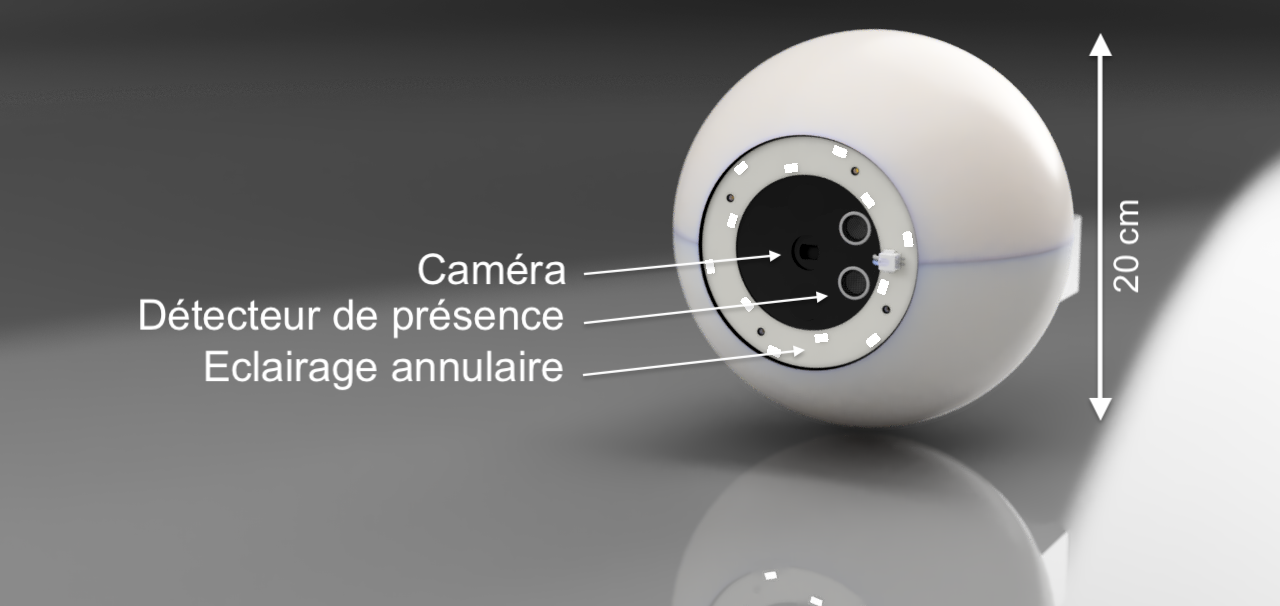
\includegraphics[width=\textwidth,height=\textheight,keepaspectratio]{../Chap5/Figures/Rendu_TE-1_2019-Jan-23_06-00-31PM_withText.png}
	\caption{Rendu réaliste du dispositif de mesure proposé.}
	\label{fig:design}
\end{figure}

\begin{figure}[hbtp]
	\centering
	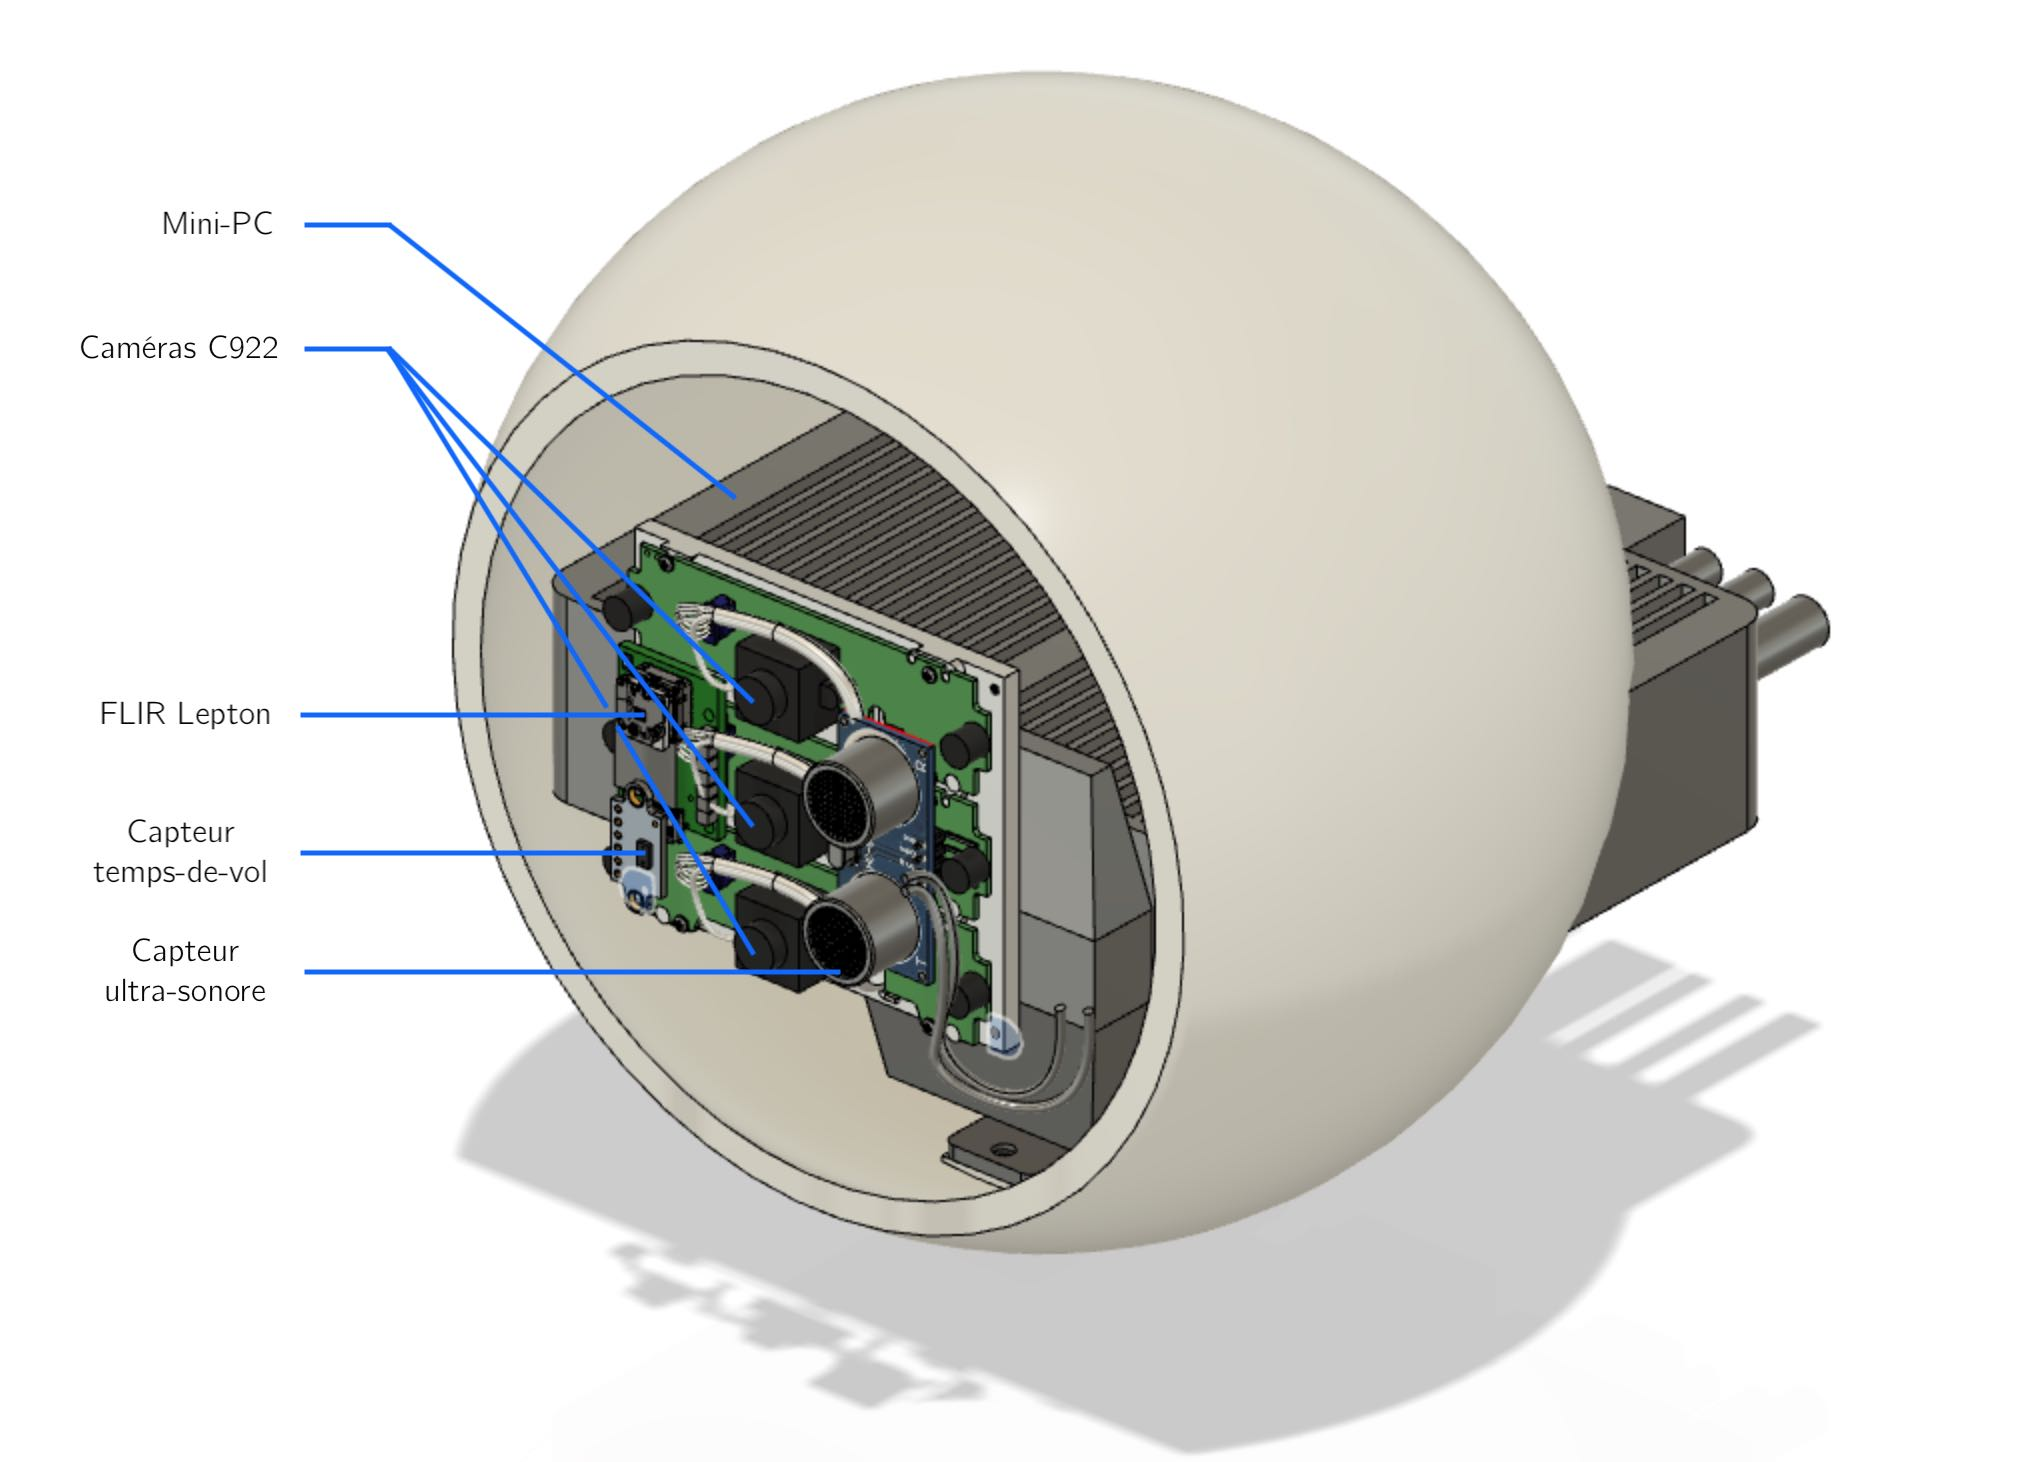
\includegraphics[width=\textwidth,height=\textheight,keepaspectratio]{../Chap5/Figures/Capture-2019-11-05-11-59-31-copie.jpg}
	\caption{Intégration des capteurs.}
	\label{fig:integration}
\end{figure}

Les caméras C922 sont des webcams destinées au grand public.
Un filtre polarisant linéaire a été positionné devant chacune d'elles, afin de réaliser un polarimètre, tel que décrit dans la Section \ref{subsec:polarimetry} du Chapitre \ref{ch:measure}.
Un éclairage annulaire linéairement polarisé, d'une intensité lumineuse de 8000 lumens est intégré autour des caméras.
L'une des caméras du système image la lumière réfléchie qui est polarisée selon un angle de 0° par rapport à l'angle de polarisation de l'éclairage ; une autre caméra à 90° ; une dernière à 120°.
Enfin, un capteur de présence de pièces est aussi intégré.

Le traitement logiciel est réalisé dans un mini-PC et les communications avec l'interface utilisateur sont réalisées par une interface réseau sans-fil \textit{WiFi}.

\FloatBarrier
\subsubsection{Détection robuste de pièces}
Afin de déclencher la mesure, il est nécessaire de savoir de manière fiable si une pièce est présente devant le dispositif.
Nous avons volontairement souhaité concevoir un système autonome, indépendant de l'automate de la ligne de production.
C'est pourquoi nous n'utilisons pas les informations de l'automate qui commande la presse et le robot de déchargement.

Un capteur de présence permet d'allumer l'éclairage et de déclencher l'enregistrement des images lorsque une pièce est présente devant le dispositif.
Pour la détection de présence, nous avons retenu trois technologies :
\begin{itemize}
	\item l'écho ultra-sonore de type sonar,
	\item la mesure d'une distance à l'aide d'un capteur laser, temps-de-vol,
	\item l'analyse d'images, en particulier l'image thermique des pièces chaudes.
\end{itemize}

\noindent
Malgré les multiples capteurs, il est possible que des images soient enregistrées alors qu'aucune pièce n'est présente (voir la Figure \ref{fig:po_trial}).
Dans ce cas, lors de la notation du jeu de données, l'expert humain peut ne pas annoter la pièce.
Une pièce non annotée n'est pas prise en compte dans le jeu de données d'apprentissage.

\subsubsection{Intégration du dispositif à la ligne de production}
Le dispositif de mesure est positionné dans la chaîne de production (voir la Figure \ref{fig:theeye_situation}).
La mesure est effectuée de manière non invasive, ni pour le procédé de fabrication, ni pour la pièce.
C'est à dire que le travail d'intégration du système à la ligne de production est minimal.
Le système est indépendant de l’outillage.
Un trépied photographique supporte le dispositif de mesure.
La pièce à contrôler est positionnée à une distance de vingt à cent centimètres du dispositif.

\begin{figure}[hbtp]
	\centering
	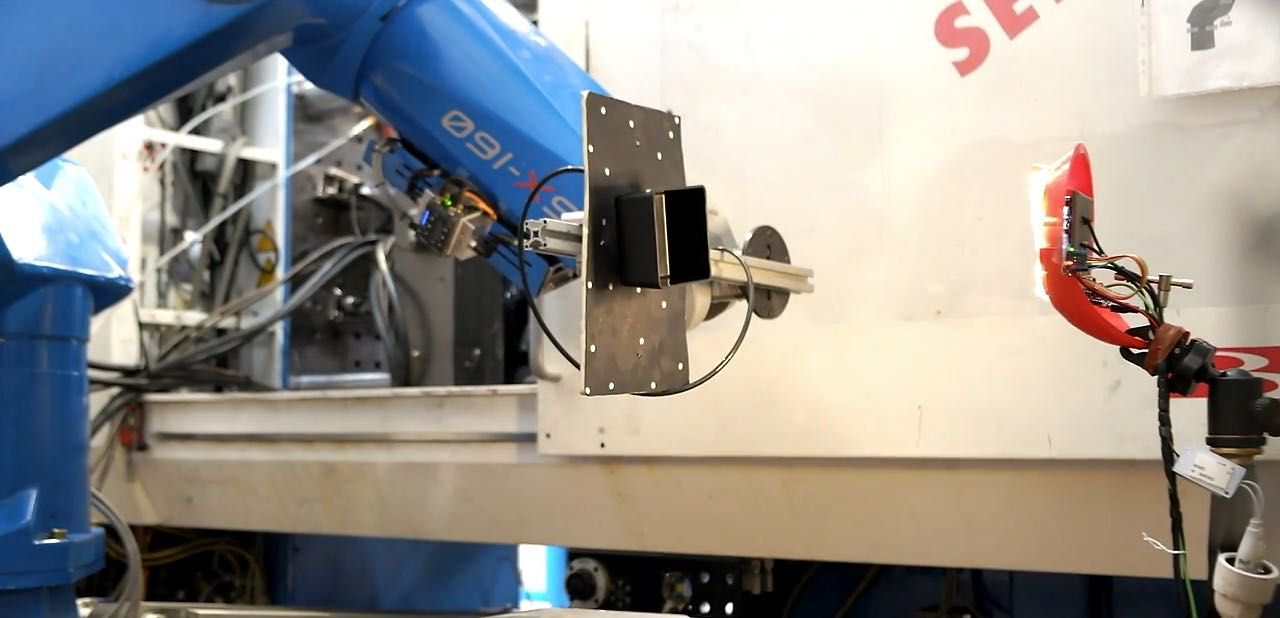
\includegraphics[width=\textwidth,height=\textheight,keepaspectratio]{../Chap5/Figures/TheEye_on.jpg}
	\caption[Photographie de la mesure d'une pièce par notre système]{Photographie de la présentation, par le bras robot, d'une pièce devant le prototype du dispositif de mesure, lors de l'essai §\ref{subsec:box_trial}.}
	\label{fig:theeye_situation}
\end{figure}

\FloatBarrier
\subsection{Solution logicielle d'analyse d'image pour inférer la qualité}
L’intégration entre les capteurs matériels et la solution logicielle permet d’obtenir un moyen de contrôle qui répond aux contraintes industrielles.
Trois grandes tâches sont réalisées à l'aide de la solution logicielle :
\begin{itemize}
	\item la classification de la qualité des pièces à partir des images,
	\item l'annotation de la qualité des pièces par l'expert humain,
	\item la mise à jour du modèle par apprentissage à partir des annotations.
\end{itemize}

Le logiciel réalise la fusion des données des capteurs et l’extraction de l’information pertinente, afin de déterminer la conformité de la pièce.

\subsubsection{Architecture logicielle}
La Figure \ref{fig:architecture} présente l'architecture logicielle du système qui s'appuie sur le principe du client-serveur.
Le dispositif de mesure acquière quatre images (1) qui sont compressées puis téléversées sur le serveur de traitement (2).
Le serveur de traitement (2) réalise l'inférence de la qualité à partir des images, à l'aide d'un modèle à réseau de neurones de convolution profond (3).
Le serveur centralise la base de données (4) et les images qui constituent le jeu de données d'apprentissage.

Lorsque le nombre d'échantillons à suffisamment augmenté dans le jeu de données d'apprentissage (4), le modèle (3) est mis à jour par ajustement des poids du réseau de neurones.
En pratique, une mise à jour toutes les cent nouvelles pièces est satisfaisante.

\begin{figure}[tbh]
	\centering
	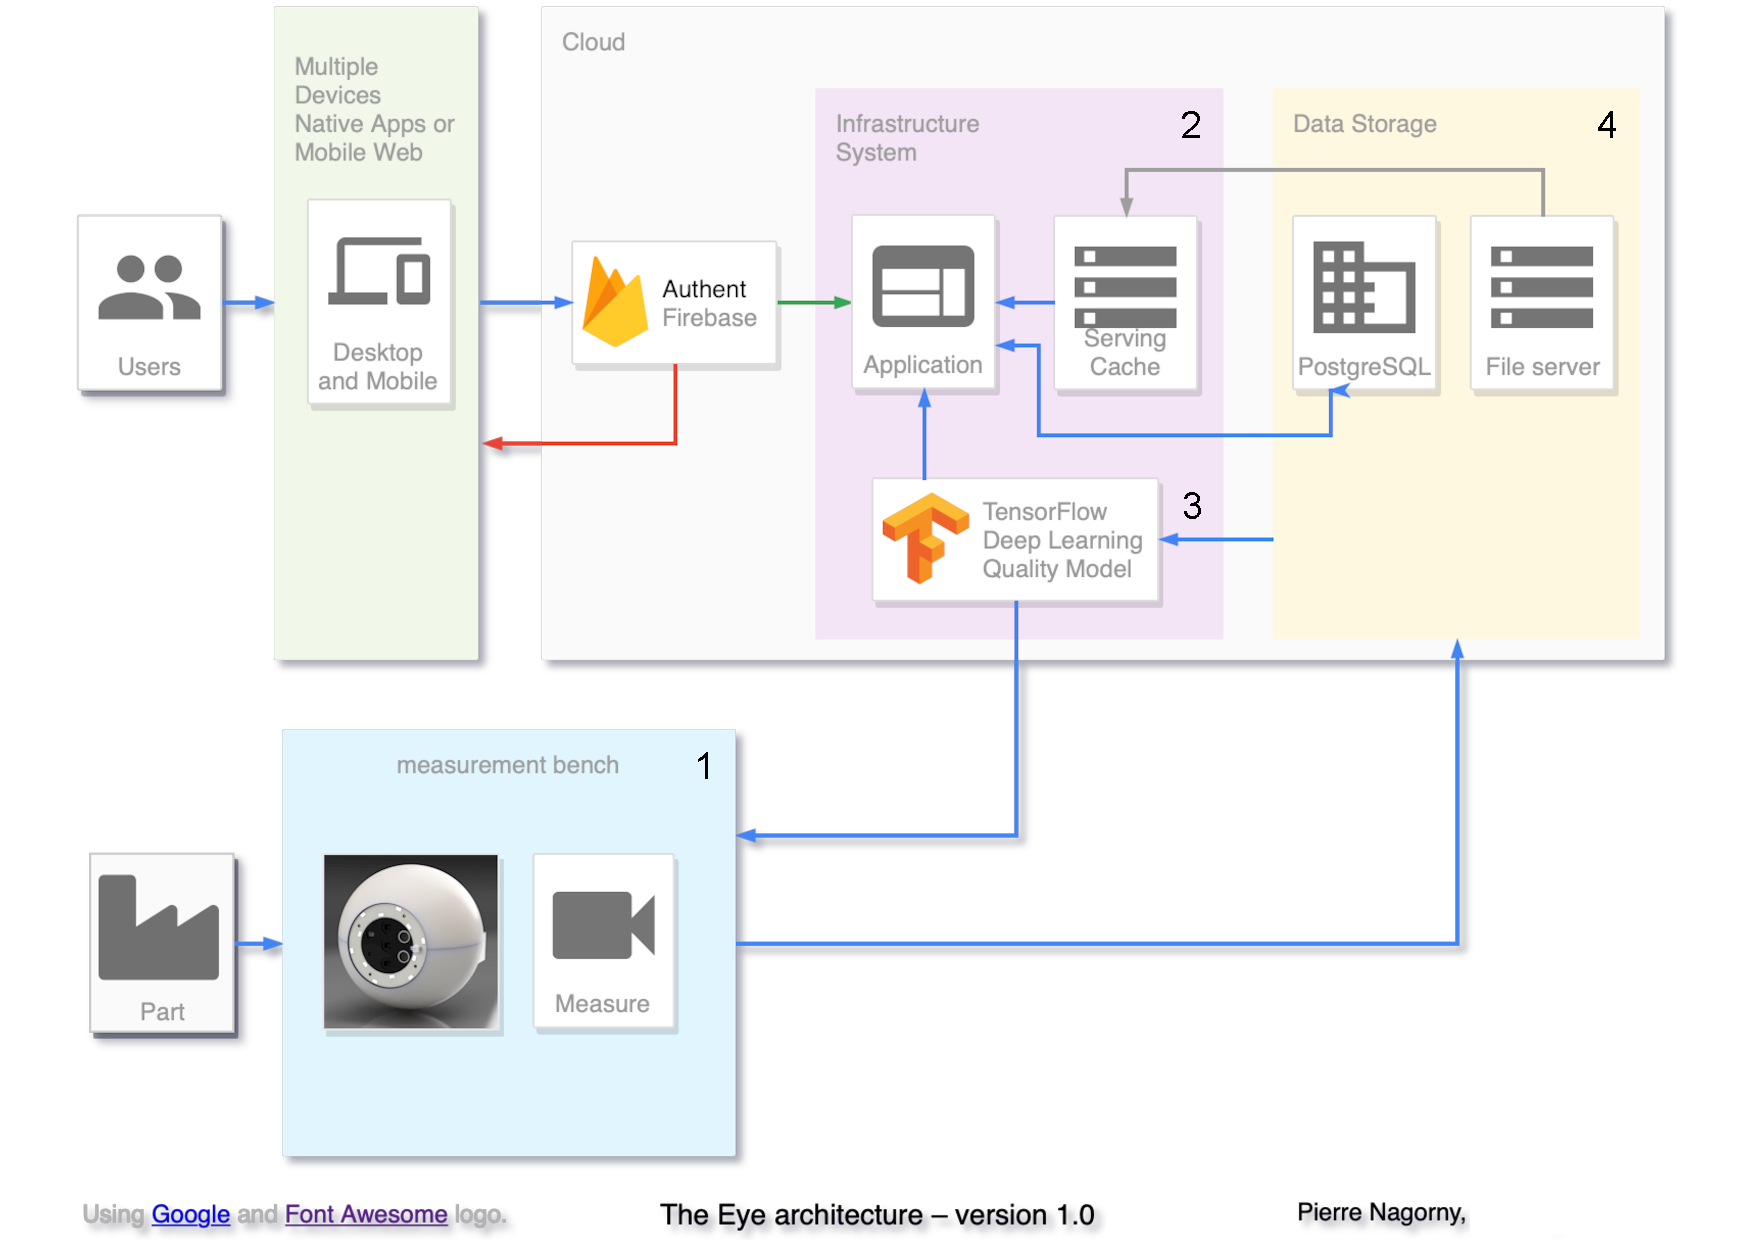
\includegraphics[width=\textwidth,height=\textheight,keepaspectratio]{../Chap5/Figures/TE_architecture.pdf}
	\caption{Architecture logicielle du système proposé.}
	\label{fig:architecture}
\end{figure}

La base de données (4) et le logiciel de traitement (2) peuvent être hébergés de manière \textit{serverless} dans le Cloud.
La principale limite est le temps de latence de la connexion réseau Internet qui nécessite une infrastructure rapide.
Dans le cas où l'environnement industriel ne permet pas cette connexion rapide, le serveur de traitement peut être installé dans l'atelier de production.

Les communications entre le client et le serveur sont réalisées par requêtes HTTP à l'aide d'une API à l'architecture REST (\textit{REpresentational State Transfer}) \cite{fielding_architectural_2000}.
Cela permet une robustesse aux erreurs de communication.
L'horodatage et l'identification de chaque pièce est sérialisé à partir d'un serveur de référence temporel NTP (\textit{Network Time Protocol}).
Enfin, le système utilise la plateforme d'authentification et de gestion des comptes utilisateurs \textit{Firebase}\footnote{\href{https://firebase.google.com/}{Site Internet} de la plateforme développée par la société Firebase.}.

\FloatBarrier
\subsubsection{Réseau de neurones pour le traitement des données} \label{neural_fusion}
La notion de qualité est spécifique à une pièce, à un cahier des charges et à une interprétation de ce cahier des charges par l’humain.
L’utilisation de l’apprentissage supervisé permet de construire une métrique de la qualité à partir de l’expertise humaine.
Cette métrique est spécifique à une pièce.
Une perspective sera de généraliser cette métrique à toutes pièces, lorsque la quantité et la diversité des pièces présentes dans le jeu de données sera suffisantes (plusieurs millions de pièces).

Nous proposons d'utiliser un unique réseau de neurones de convolution pour réaliser l'extraction de l'information et la fusion des données issues des quatre caméras.
% L'utilisation d'un réseau de convolution profond permet de réaliser l'extraction de l'information pertinente et la fusion des données issues de multiples capteurs.

\paragraph{4.1.2.2.1 Fusion multi-modale et transfert de domaine} \mbox{} \\
Dans notre contexte industriel, la quantité de pièces d'apprentissage dont nous disposons est trop faible pour réaliser l'apprentissage d'un réseau de convolution profond complet.
C'est pourquoi notre approche est de réaliser un apprentissage par transfert de domaine\footnote{Nous discutons du principe de l'apprentissage par transfert de domaine dans l'Annexe \ref{subsec:transfer_learning}. Cela consiste à utiliser d'autres jeux de données d'images.}.
Nous utilisons le réseau de neurones profond, pré-appris sur un jeu de données différents qui dispose d'un grand nombre d'individus (\textit{ImageNet} possède 2 millions d'images pour 1000 catégories).

L'architecture du réseau de neurones que nous utilisons est constituée de quatre réseaux résiduels\footnote{Nous détaillons le principe des blocs résiduels dans l'Annexe \ref{subsubsec:ResNet}.} \textit{DenseNet} \cite{huang_densely_2016} parallèles, représentée dans la Figure \ref{fig:transferdensenet121}.
Nous utilisons la librairie TensorFlow \cite{abadi_tensorflow_2016} pour construire le réseau et réaliser l'apprentissage par optimisation des poids.
Le réseau \textit{DenseNet} est tronqué au niveau de son avant-dernière couche \textit{conv4}.
Chaque réseau prend en entrée les données brutes issues de chacune des quatre caméras du dispositif de mesure.
À la suite, les quatre réseaux sont fusionnés par concaténation des valeurs scalaires en sortie de la couche \textit{conv4}.
Deux couches pleinement connectées, et une fonction d'activation sigmoïde \footnote{La fonction d'activation \textit{sigmoïde} est discutée dans la Section \ref{eq:sigmoid}.} transforment enfin ces valeurs en une probabilité de conformité de la pièce.
Les hyper-paramètres de ces deux dernières couches sont optimisés automatiquement par validation croisée\footnote{Nous détaillons le principe de la validation croisée dans l'Annexe \ref{subsubsec:cross_val}.}.

%\begin{figure}
%	\centering
%	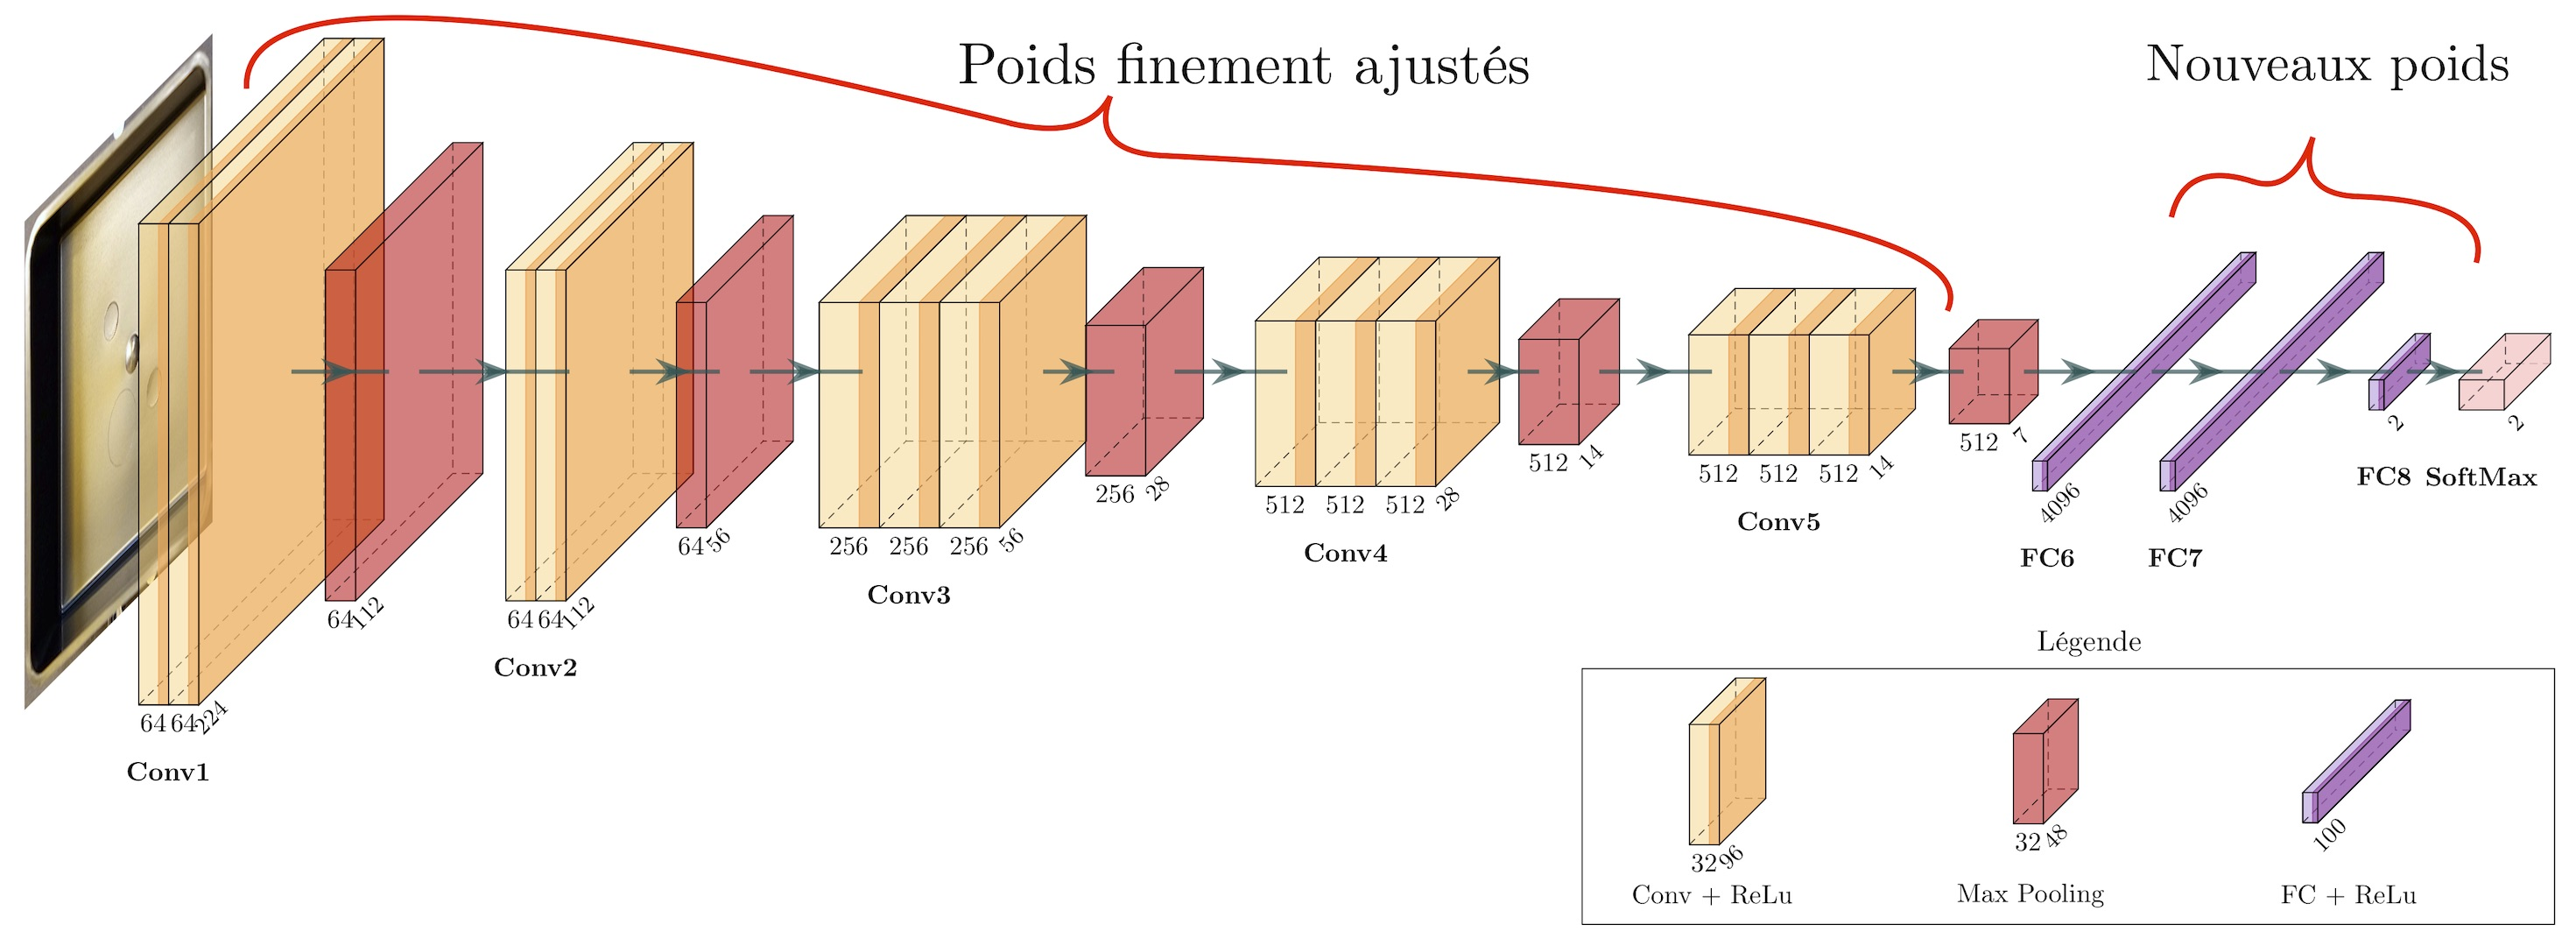
\includegraphics[width=\textwidth,height=\textheight,keepaspectratio]{../Chap5/Figures/transfer_VGG16.jpg}
%	\caption{Apprentissage par transfert de domaine.}
%	\label{fig:transfervgg16}
%\end{figure}

\begin{figure}[hbtp]
	\centering
	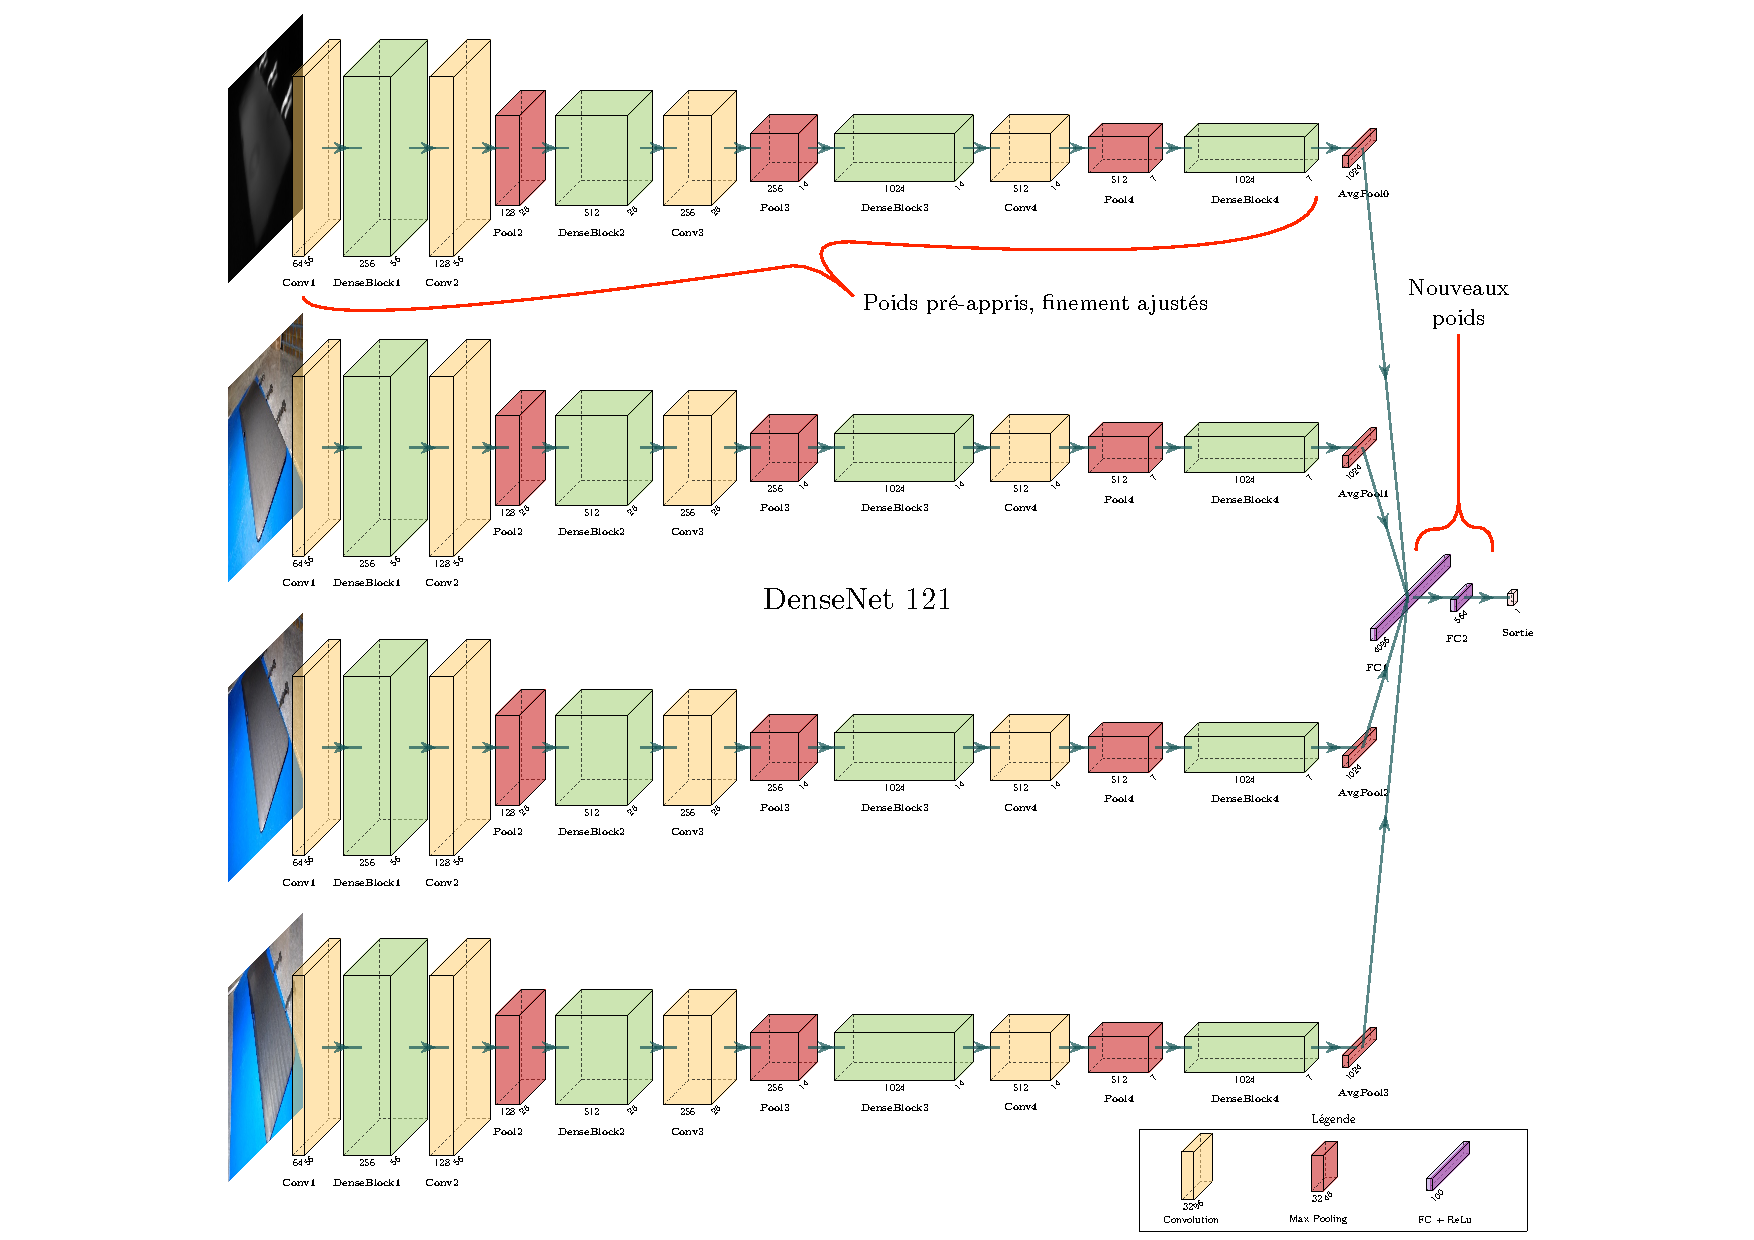
\includegraphics[width=\textwidth,height=\textheight,keepaspectratio]{../Chap5/Figures/transfer_densenet121.pdf}
	\caption{Apprentissage par transfert de domaine à partir du réseau \textit{DenseNet121} pré-appris sur \textit{ImageNet}.}
	\label{fig:transferdensenet121}
\end{figure}

% \subsection{Apprentissage de la notion de Qualité}
%TODO: Eric: masse d'informations
% - Des capteurs partout
% - Des caméras thermiques, mais l'humain n'est pas capable de les exploiter.
% - IA = information synthétisée, exploitée

\paragraph{4.1.2.3.2 Durée de l'apprentissage du modèle} \mbox{} \\
Pour réaliser le transfert de domaine, dans un premier temps, seuls les poids des dernières couches du réseau \textit{FC1} et \textit{FC2} sont ajustés\footnote{On parle d'"apprentissage du réseau". Nous avons détaillé le principe de l'apprentissage par optimisation itératif des poids (la rétro-propagation du gradient de l'erreur de classification) dans l'Annexe \ref{subsubsec:deep_learning}.}.
Ensuite, l'ensemble des poids du réseau est ajusté.
Le critère d'optimisation des poids est la minimisation de l'erreur de justesse balancée\footnote{La métrique de justesse balancée est discutée dans la Section \ref{eq:balanced_accuracy}.}.

Le nombre d'individus du jeu de données est très faible.
C'est pourquoi nous utilisons la méthode d'augmentation artificielle du jeu de données\footnote{La méthode d'augmentation artificielle du jeu de données est présenté dans l'Annexe \ref{parag:data_augmentation}.}.
Les images sont aléatoirement recadrées de 10\% de leurs dimensions et une rotation de 0° à 10° est appliquée.
Ces transformations aléatoires permettent de rendre robuste le réseau aux variations de position des pièces.
Elles sont représentatives de notre cas d'application, où les pièces sont positionnées de manière relativement répétable.

Nous utilisons une validation croisée\footnote{La méthode de validation croisée est présentée dans l'Annexe \ref{subsubsec:cross_val}.}.
C'est pourquoi le jeu de données est divisé en deux sous-ensembles : un ensemble d'apprentissage composé de 60\% des pièces et un ensemble de validation composé de 40\% des pièces.
Afin de limiter le sur-apprentissage, la technique d'arrêt prématuré\footnote{La technique de l'arrêt prématuré est une méthode de régularisation qui est détaillée dans l'Annexe \ref{parag:early_stopping}.} est employée.
Si l'erreur de justesse ne diminue pas pendant plus de trente itérations, l'apprentissage est arrêté et les poids du réseau sont conservés.

La Figure \ref{fig:learning} présente l'évolution, au cours de l'apprentissage, de l'erreur de justesse pour le jeu de données d'apprentissage et pour le jeu de données de validation.
Cette Figure est réalisée à l'aide du jeu de données "boîtes noires", présenté dans la Section \ref{subsec:box_trial} suivante.
L'apprentissage est réalisé avec un processeur graphique \textit{NVIDIA GTX 1080Ti} pour accélérer les calculs massivement parallèles.
Nous observons en (a) une diminution rapide de l'erreur de justesse lors de l'apprentissage initial des dernières couches du réseau.
Cette première phase est également rapide, d'une durée totale de six secondes.
En (b), nous observons l'évolution lors de l'apprentissage de spécialisation de l'ensemble du réseau.
La convergence est plus lente (quatre-vingt deux secondes) et le nombre d'individus du jeu de données limite l'amélioration de la performance.
La durée totale de l'apprentissage est de cent secondes.

\begin{figure}[hbtp]
	\centering
	\begin{subfigure}[c]{0.75\textwidth}
		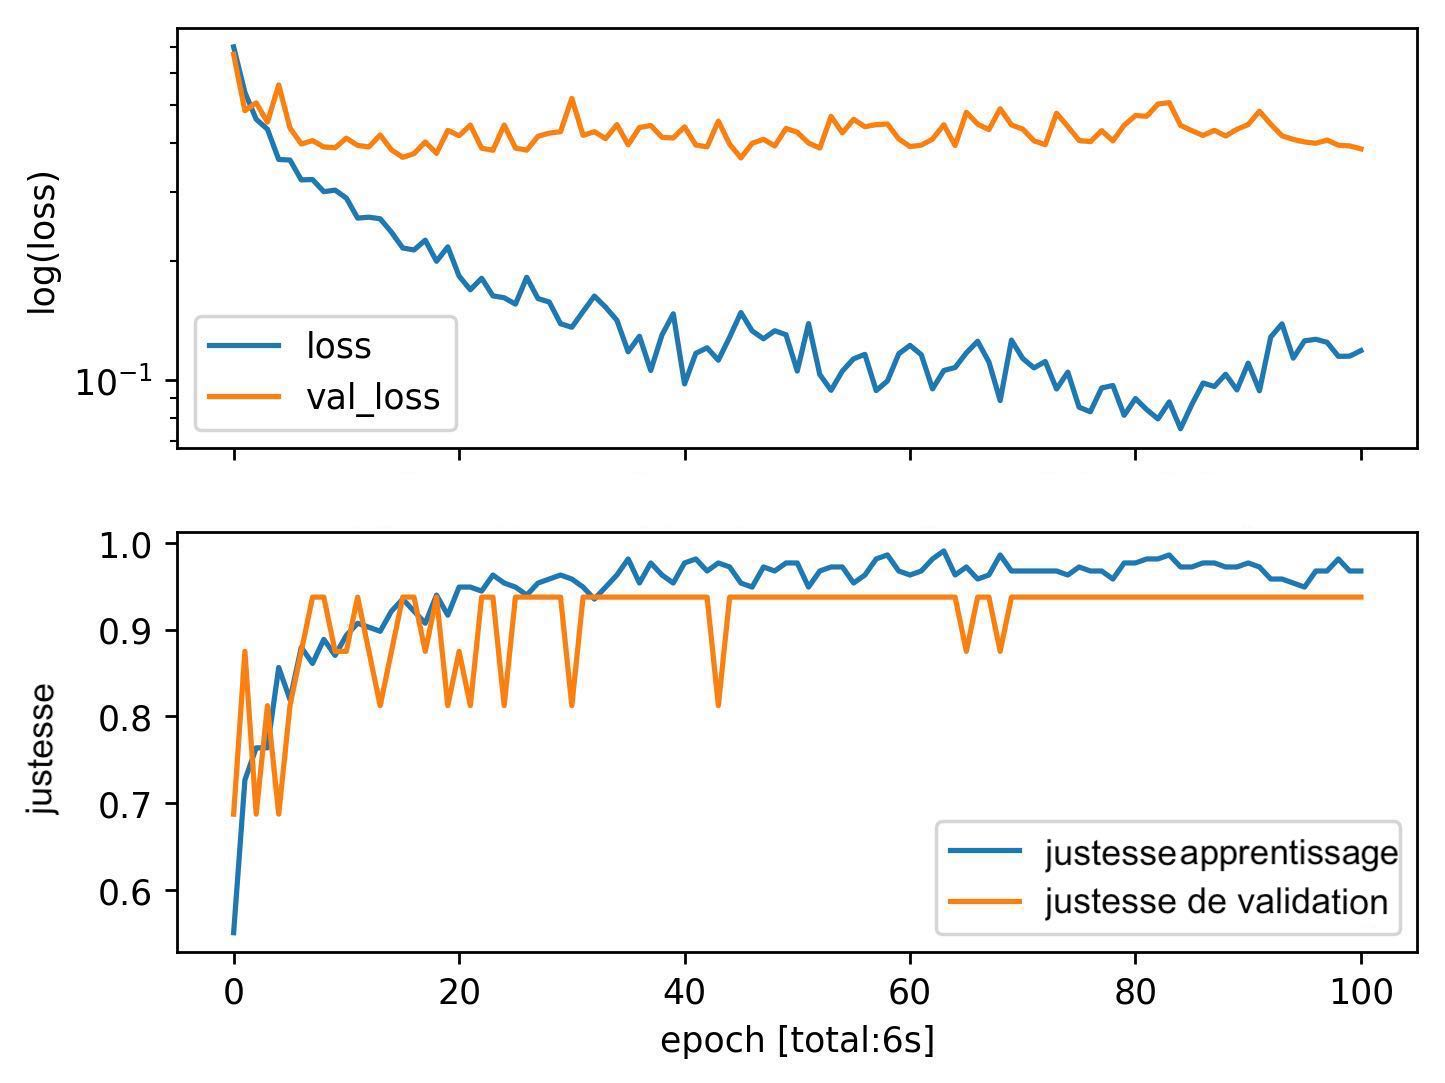
\includegraphics[width=\textwidth]{../Chap5/Figures/8_photo_Qtotal_crop_DNN_top_model_training.jpg}
		\caption{Apprentissage initial des dernières couches du réseau.}
		\vspace*{5mm}
	\end{subfigure}
	\\
	\begin{subfigure}[c]{0.75\textwidth}
		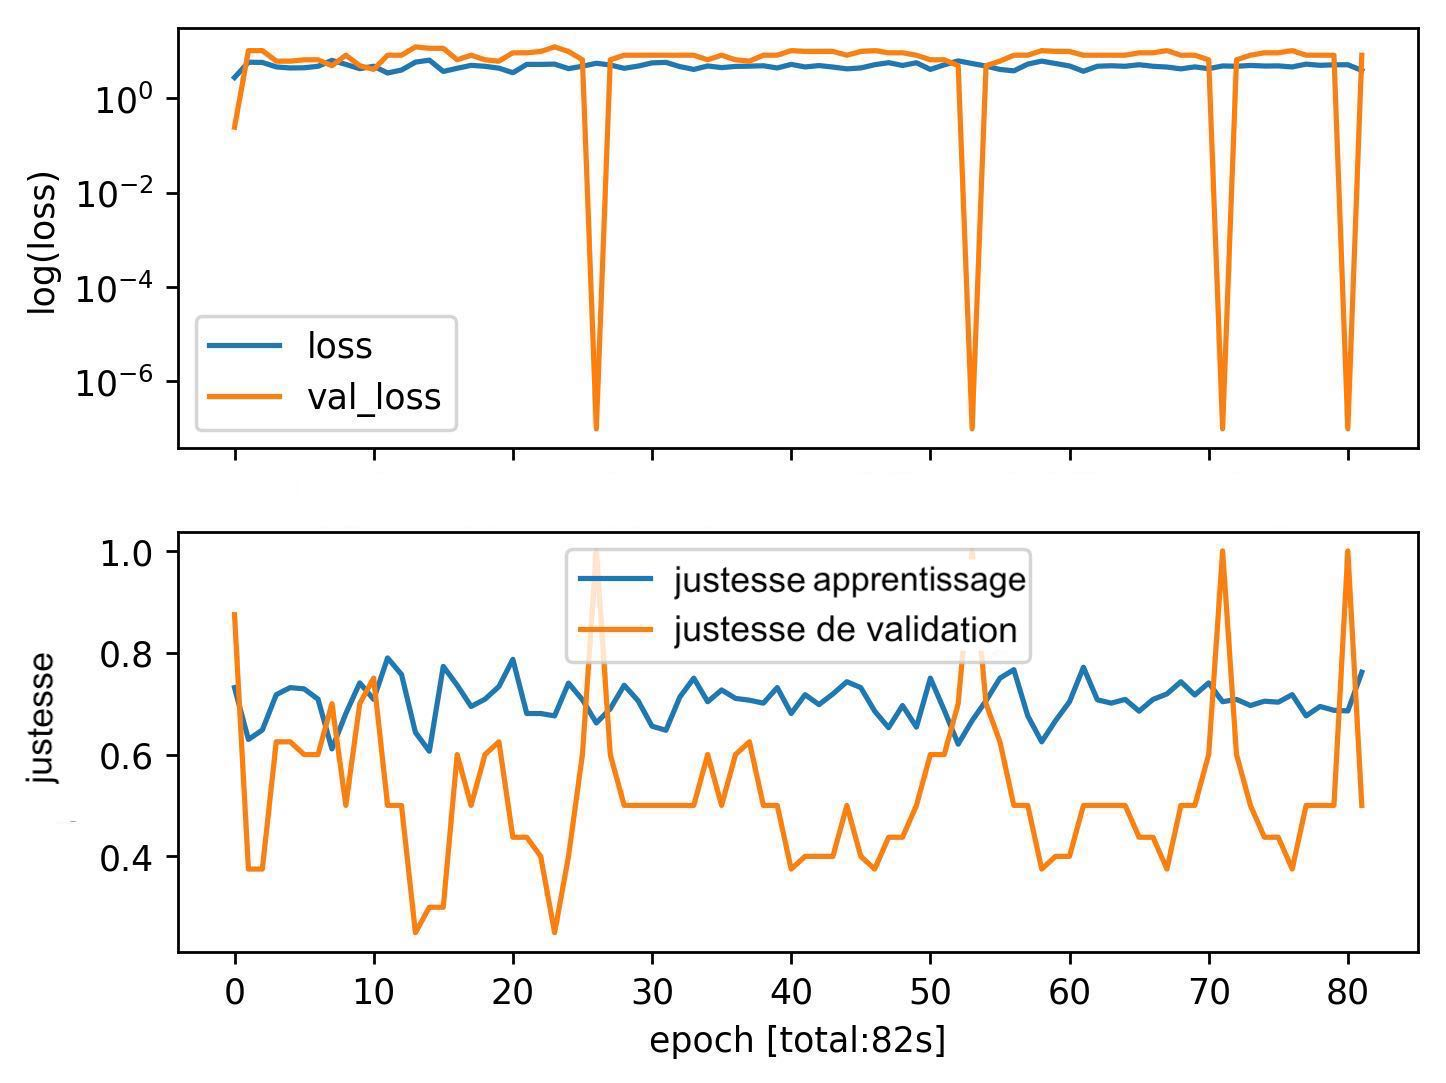
\includegraphics[width=\textwidth]{../Chap5/Figures/9_photo_Qtotal_crop_DNN_full_model_fine-tuning.jpg}
		\caption{Apprentissage de spécialisation de l'ensemble des poids du réseau.}
	\end{subfigure}
	\caption{Évolution de l'erreur de prédiction et de la justesse balancée de classification, pendant l'apprentissage des poids du réseau.}
	\label{fig:learning}
\end{figure}

\paragraph{4.1.2.3.3 Optimisation automatique du réseau de neurones} \mbox{} \\
L'architecture du réseau \textit{DenseNet} ne peut pas être modifiée car les poids du réseau ont été précédemment appris sur le jeu de données \textit{ImageNet}.
Nous avons choisi d'optimiser l'architectures des dernières couches du réseau de neurones, ainsi que les hyper-paramètres, par optimisation bayésienne, à l'aide de la méthode \textit{BOHB}\footnote{Nous présentons la méthode \textit{BOHB} dans la Section \ref{subsec:bandit} du chapitre précédent.} (\textit{Bayesian Optimization and HyperBand}).

La durée de l'apprentissage du modèle est relativement courte, ce qui nous permet de réaliser cette optimisation des hyper-paramètres.
Les performances de soixante-dix modèles différents sont évalués pendant deux heures.
Les hyper-paramètres du meilleur modèle sont ensuite utilisés pour réaliser la classification.
Le nombre de neurones optimal pour la couche pleinement connectée \textit{FC2} est de 522.
Une fonction d'activation \textit{ReLu}\footnote{La fonction d'activation \textit{ReLu} est discutée dans la Annexe \ref{subsubsec:activation}.} est utilisée.
%TODO: which hyperparamters are tuned?

%\paragraph{Fusion de multiples capteurs}
%Nous avons évalué trois démarches de fusion : la fusion des données brutes dès l'entrée du réseau, la fusion à l'avant-dernière couche du réseau et la fusion lors de la dernière couche du réseau.
%Les meilleurs performances furent obtenues pour la fusion lors de l'avant-dernière couche.

\FloatBarrier
\subsubsection{Interface utilisateur d'annotation en ligne de production} \label{subsubsec:hmi}
% Interface web based
% API REST
% Les pages sont générées à partir de système de template du framework ask.
Notre logiciel propose une interface utilisateur pour réaliser l'annotation des pièces dans le cadre de l'apprentissage supervisé.
Elle est destinée à être utilisée par un technicien-régleur ou un expert qualité.
Dès qu'une pièce est produite et imagée, elle s'affiche dans l'interface en surimpression, telle que présentée dans la Figure \ref{fig:hmi}.

\begin{figure}[hbt!]
	\centering
	\begin{subfigure}[c]{0.60\textwidth}
		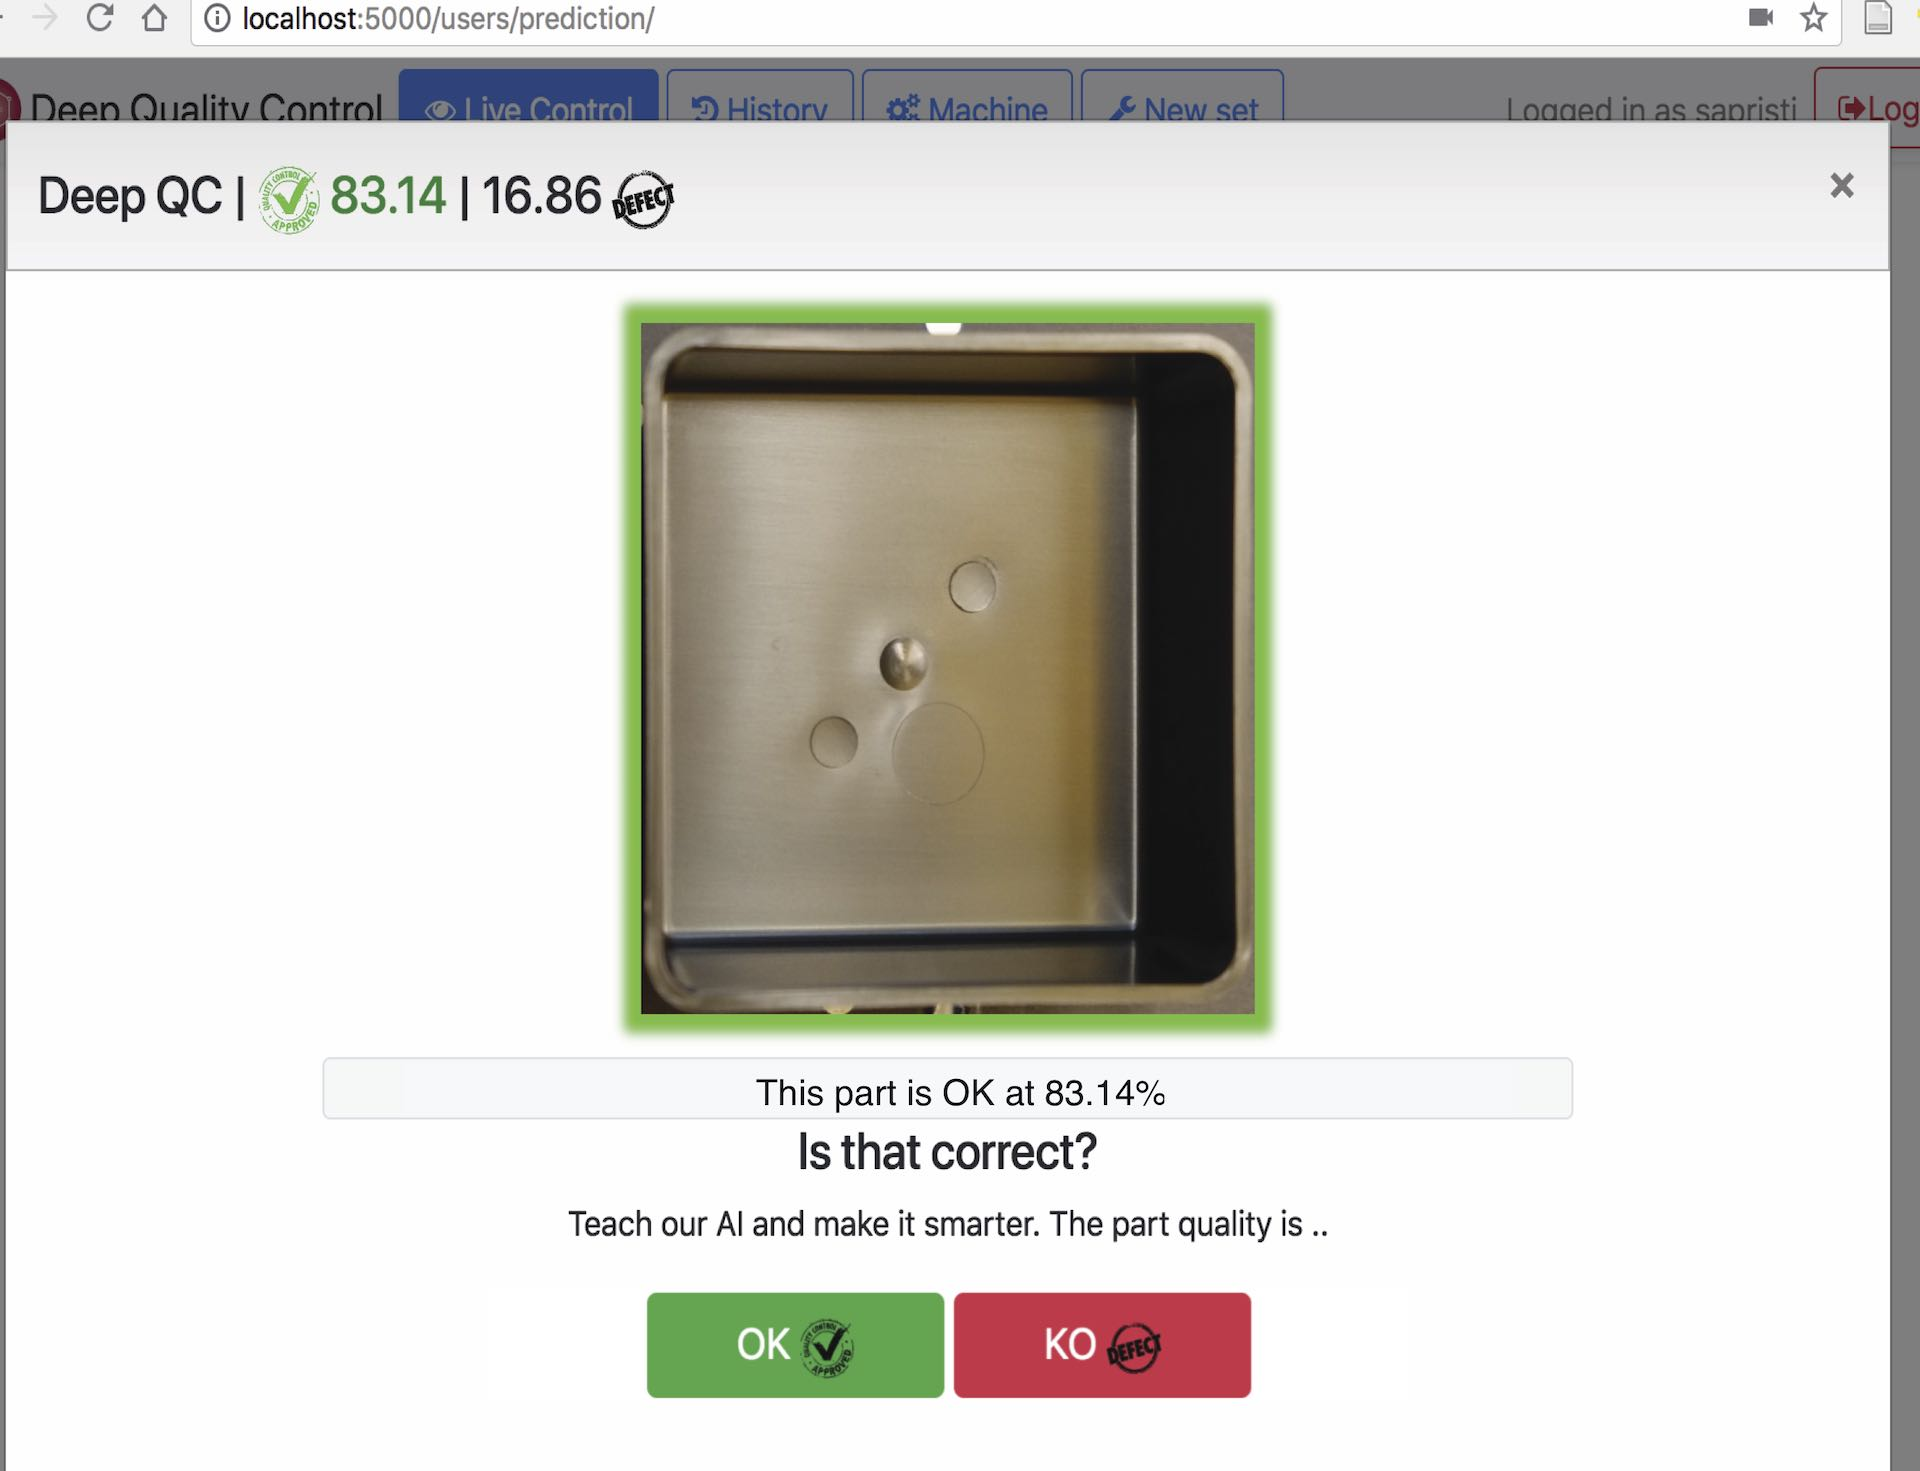
\includegraphics[width=\textwidth]{../Chap5/Figures/annotation_hmi.jpg}
		\caption{Annotation de la qualité au fur et à mesure de la production.}
	\end{subfigure}
	\\
	\bigskip
	\begin{subfigure}[c]{0.60\textwidth}
		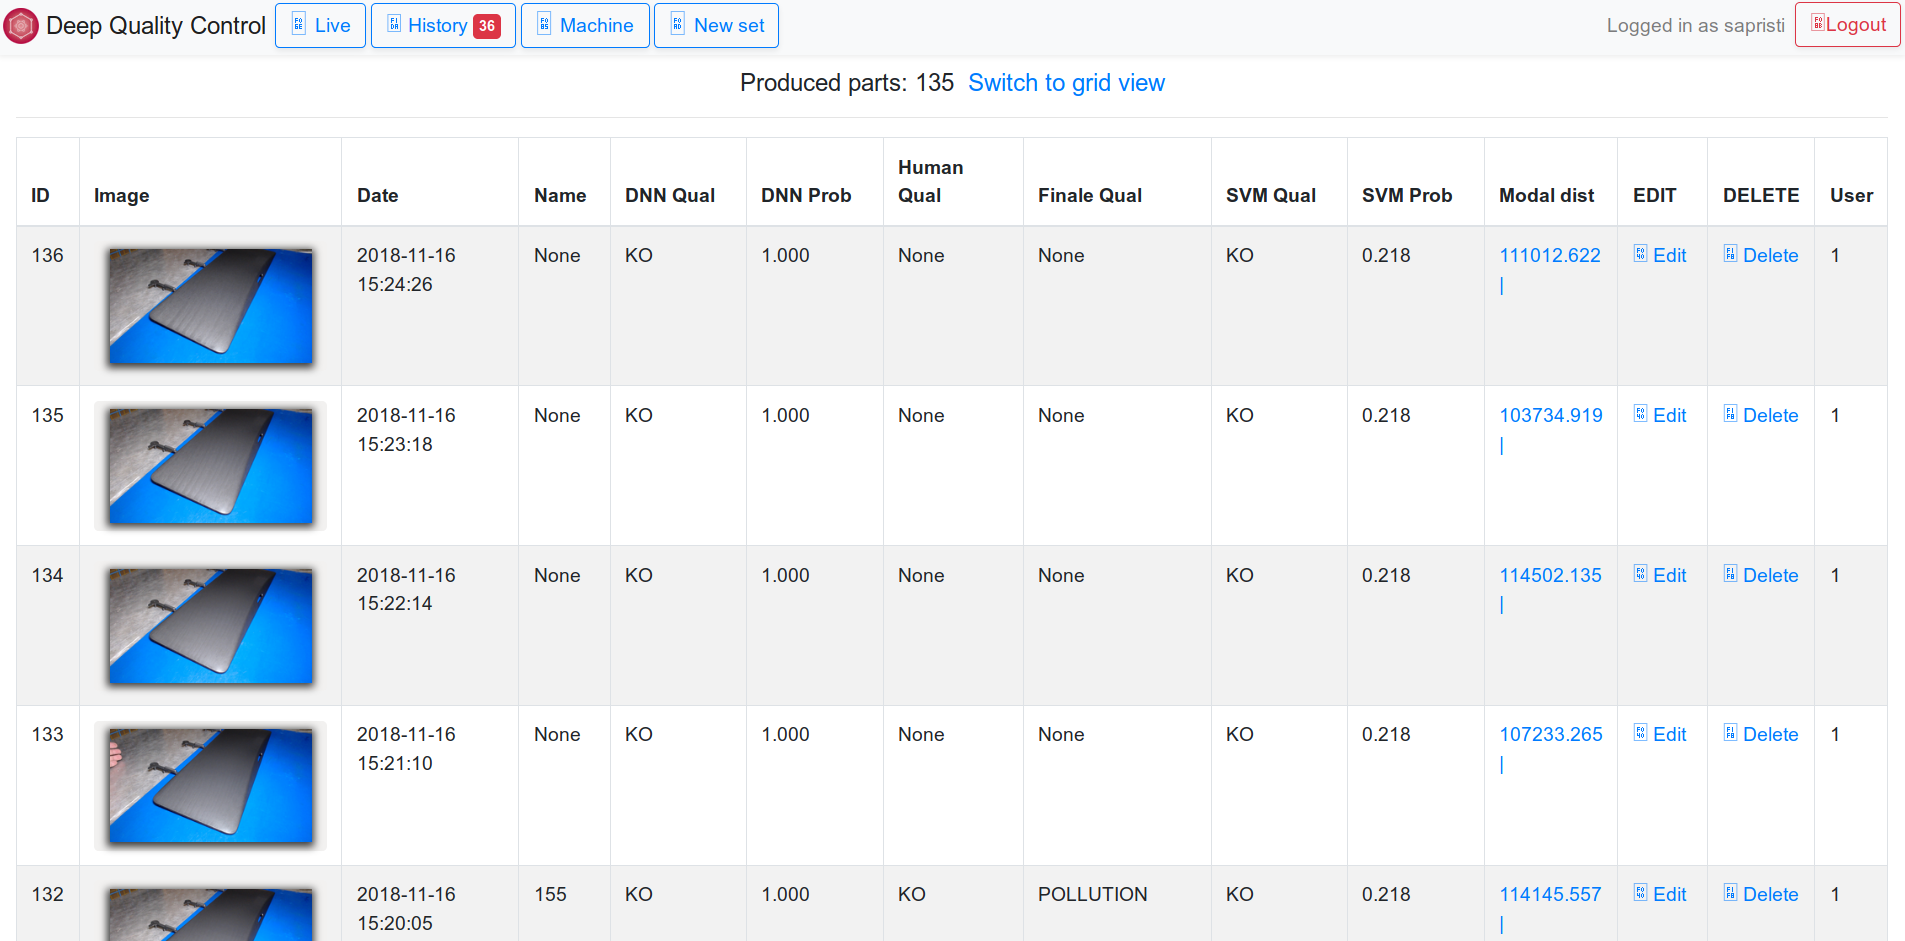
\includegraphics[width=\textwidth,height=\textheight,keepaspectratio]{../Chap5/Figures/Capture-2018-11-21-15-10-59.png}
		\caption{Historique de la production et annotations associées.}
		\vspace*{5mm}
	\end{subfigure}
	\caption{Interface utilisateur d'annotation de la conformité des pièces.}
	\label{fig:hmi}
\end{figure}

% L’expert qualité et l’opérateur sont au cœur de ce système, c’est pourquoi il est important de leur proposer une interface agréable et une procédure d’utilisation la plus simple possible.

L'utilisateur voit la classification de la pièce réalisée par le modèle sous la forme d'une message et d'un code couleur (vert pour une pièce conforme, rouge pour une pièce non-conforme).
La confidence de la décision est affichée en pourcentage.
C'est la valeur de la probabilité de conformité qui est retournée par la dernière couche \textit{SoftMax} du réseau.
% Le système propose à l'utilisateur de classer la pièce comme conforme ou non, à partir de son modèle.
L'utilisateur peut alors accepter ou modifier l'annotation de la pièce.
Lorsque qu'une annotation d'une pièce a été validée par l'utilisateur, les images sont ajoutées au jeu de données d'apprentissage.
% Si l'utilisateur constate une erreur de classification du modèle, il peut modifier la catégorie de la pièce.
% L'utilisateur peut également confirmer la catégorie de la pièce.
% Dans ces cas, la pièce est ajoutée au jeu de données d'apprentissage.

Nous n'ajoutons pas automatiquement toutes les pièces au jeu de données d'apprentissage afin d'éviter les erreurs d'annotations et les biais.
Ainsi, au début de l'utilisation de notre système, la base d'apprentissage ne contient pas de pièces annotées.
L'utilisateur doit alors annoter des pièces pour que le modèle soit mis à jour.
Dès qu'une vingtaine de pièces sont présentes dans le jeu de données, l'apprentissage débute.
Cent secondes plus tard, le modèle peut prédire la qualité.
Par la suite, l'utilisateur affine le modèle au fur et à mesure de la production.

\textit{A posteriori} de la production des pièces, l'utilisateur peut également modifier la catégorie des pièces et ainsi augmenter la quantité de pièces dans le jeu de données d'apprentissage.
L'interface est accessible depuis un navigateur web, sur station de travail, tablette ou smartphone.
Lorsque vingt nouvelles pièces ont été ajoutées, l'apprentissage du modèle est réalisé pour améliorer la performance de classification de la conformité.

\miniconclusion{Synthèse : Système de contrôle par apprentissage et imagerie non-conventionnelle}{
	Nous proposons un système de contrôle qui utilise l'apprentissage statistique afin de déterminer si la pièce est conforme ou non.
	Le système se compose d'un dispositif de mesure qui enregistre quatre images pour chaque pièce produite : une image thermique et trois images polarisées linéairement à des angles de 0°, 45° et 90°.

	Une réseau de neurones profond analyse ces quatre images et retourne une probabilité de conformité.
	Le réseau de neurones utilise un apprentissage par transfert de domaine, à partir d'un réseau pré-appris sur une grande quantité de données.

	Une interface utilisateur dans un navigateur web permet à l'utilisateur, technicien-régleur ou expert qualité, d'apprendre au système si les pièces sont conformes ou non.
	L’humain est au cœur de ce système, c’est pourquoi il est important proposer une interface agréable et ergonomique.
	Chaque nouvelle pièce enregistrée par le système est affichée dès sa production.
	L'interface affiche le degré de conformité retourné par le système et l'utilisateur peut modifier la réponse donnée si celle-ci est erronée.

	En début de production, l'utilisateur doit annoter cent pièces pour que le système apprenne un modèle de la qualité.
	Par la suite, toutes les vingts nouvelles pièces annotées, le modèle est mis à jour.
}

\FloatBarrier
\newpage
\section{Validation expérimentale : applications industrielles} \label{sec:theeye_validation}
% \end{raggedright}

% \subsection{Démarche expérimentale}
Afin de valider les performances du système de contrôle proposé, nous avons réalisé deux expérimentations.
Notre démarche expérimentale consiste en la production d'un grand nombre de pièces et en la mesure de chacune d'elle par notre dispositif.
Les réglages de la presse à injecter sont variés au cours de l'expérimentation afin de produire des pièces dont la qualité est considéré comme conforme et des pièces non.
Pour chaque pièce, un expert humain détermine de manière binaire si la pièce est conforme ou non-conforme et renseigne cette annotation à l'aide de l'interface présenté dans la Section \ref{subsubsec:hmi} précédente.

% Pour ces expériences, l'exploration des réglages de la presse à injecter ne suit pas de plan d'expériences, à la différence de l'essai présenté dans la Section \ref{sec:experiment} du Chapitre \ref{ch:measure}.
Le jeu de données a principalement été construit pendant que le technicien-régleur effectuait les réglages de la machine.
L’opérateur humain explore généralement naturellement les réglages de la machine pour choisir le bon réglage pour produire des pièces conformes.

% \subsection{Méthode d'analyse des données}
Afin de comparer les deux expérimentions, nous utilisons une validation croisée \textit{3-folds} qui comporte 60\% des pièces du jeu de données en apprentissage et 40\% des pièces en validation.
Cette validation est réalisée trois fois en tirant aléatoirement les pièces à chaque fois.
Les performances moyennes et l'écart-type des résultats sont étudiés.
Nous présenterons les résultats de chaque expérimentation dans les deux sections suivantes.

% Nous utilisons un réseau de neurones \textit{DenseNet 121}, qui est tronqué au niveau de sa dernière couche, tel que présenté dans la Section \ref{neural_fusion}.

\subsection{Essai "boîte noire" au Centre Techniques IPC} \label{subsec:box_trial}
Cet essai a été réalisé en juin 2019 au Centre Technique IPC.
La pièce produite est une "boîte noire" de 90 $\times$ 90 mm, que nous avons également étudiée dans la Section \ref{sec:experiment}.
La matière utilisée est un polypropylène automobile \textit{ExonMobil EXXTRAL CMU201} de couleur noire.
Les pièces sont produites avec une durée de cycle de quarante secondes.
La mesure est effectuée dix secondes après la sortie du moule.
C'est la durée du convoyage par le bras robotisé.
La disposition du dispositif de mesure sur la ligne de production est présentée dans la Figure \ref{fig:theeye_situation}.

Le jeu de données obtenu est constitué de 240 séries de quatre images, qui correspondent à chacune des pièces produites.
La Figure \ref{fig:IPC_ok_ko} présente les images de la caméra linéairement polarisée selon un angle de 0°, pour une pièce conforme et une pièce non-conforme.
Lors de l'expérience, des images ont été capturées par erreur alors que la pièce n'était pas présente devant le dispositif de mesure ; ces images ont été écartées du jeu de données.

\begin{figure}[hbtp]
	\centering
	\begin{subfigure}[c]{0.49\textwidth}
		\includegraphics[width=\textwidth]{../Chap5/Figures/OK_cam_1180717163656.jpeg}
		\caption{Image d'une pièce conforme.}
	\end{subfigure}
	\begin{subfigure}[c]{0.49\textwidth}
		\includegraphics[width=\textwidth]{../Chap5/Figures/KO_cam_1180717164948.jpeg}
		\caption{Image d'une pièce non-conforme à cause d'une retassure.}
	\end{subfigure}
	\caption{Images originales pour la caméra linéairement polarisée selon un angle de 0°.}
	\label{fig:IPC_ok_ko}
\end{figure}

\subsubsection{Matrices de confusion}
Le Tableau \ref{tab:box_results} présente les matrices de confusion obtenues pour le jeu de données d'apprentissage et pour le jeu de données de validation.
\begin{table}[!h]
	\centering
	\begin{subtable}{1\textwidth}
		\centering
		\arrayrulecolor{black}\begin{tabular}{c c|c|c|}
			\cline{3-4}
			& & \multicolumn{2}{c|}{Classes vraies}               \\ \cline{3-4}
			& & \multicolumn{1}{c|}{Conformes} & \multicolumn{1}{c|}{Non-conformes} \\ \hline
			\multicolumn{1}{|c|}{\multirow{2}{*}{Classes prédites}} & Conformes & Vrais positifs : 65 & Faux Positifs : 0 \\ \cline{2-4} 
			\multicolumn{1}{|c|}{} & Non-conformes & Faux négatifs : 1  & Vrais Négatifs : 102 \\ \hline
		\end{tabular}
		\caption{Jeu de données d'apprentissage.}
	\end{subtable}

	\bigskip

	\begin{subtable}{1\textwidth}
		\centering
		\arrayrulecolor{black}\begin{tabular}{l c|c|c|}
			\cline{3-4}
			& & \multicolumn{2}{l|}{Classes vraies}               \\ \cline{3-4}
			& & \multicolumn{1}{l|}{Conformes} & \multicolumn{1}{l|}{Non-conformes} \\ \hline
			\multicolumn{1}{|l|}{\multirow{2}{*}{Classes prédites}} & Conformes & Vrais positifs : 36 & Faux Positifs : 0 \\ \cline{2-4} 
			\multicolumn{1}{|l|}{} & Non-conformes & Faux négatifs : 0  & Vrais Négatifs : 36 \\ \hline
		\end{tabular}
		\caption{Jeu de données de validation.}
	\end{subtable}
	\caption{Matrices de confusion pour l'essai boîtes noires.}
	\label{tab:box_results}
\end{table}

Le nombre d'erreurs de classification en apprentissage est très faible.
Il est nulle pour le jeu de données de validation.
Le réseau permet de classifier la conformité des pièces avec succès.

% \paragraph{4.2.1.1.2 Courbe ROC} \mbox{} \\
La Figure \ref{fig:roc_result} présente la courbe ROC
\footnote{La courbe ROC représente la performance d'un classifieur. Elle est présentée en détail dans l'Annexe \ref{subsec:roc}.} (\textit{Receiver Operating Characteristic}) obtenue pour le jeu de données de validation.
Cette courbe est calculée une fois l'apprentissage du modèle effectuée.
Elle permet de distinguer les vrais positifs des erreurs de classification (taux de vrais négatifs).
La performance est comparée à la réponse d'un classifieur aléatoire (droite rouge en pointillée).

\begin{figure}[bthp]
	\centering
	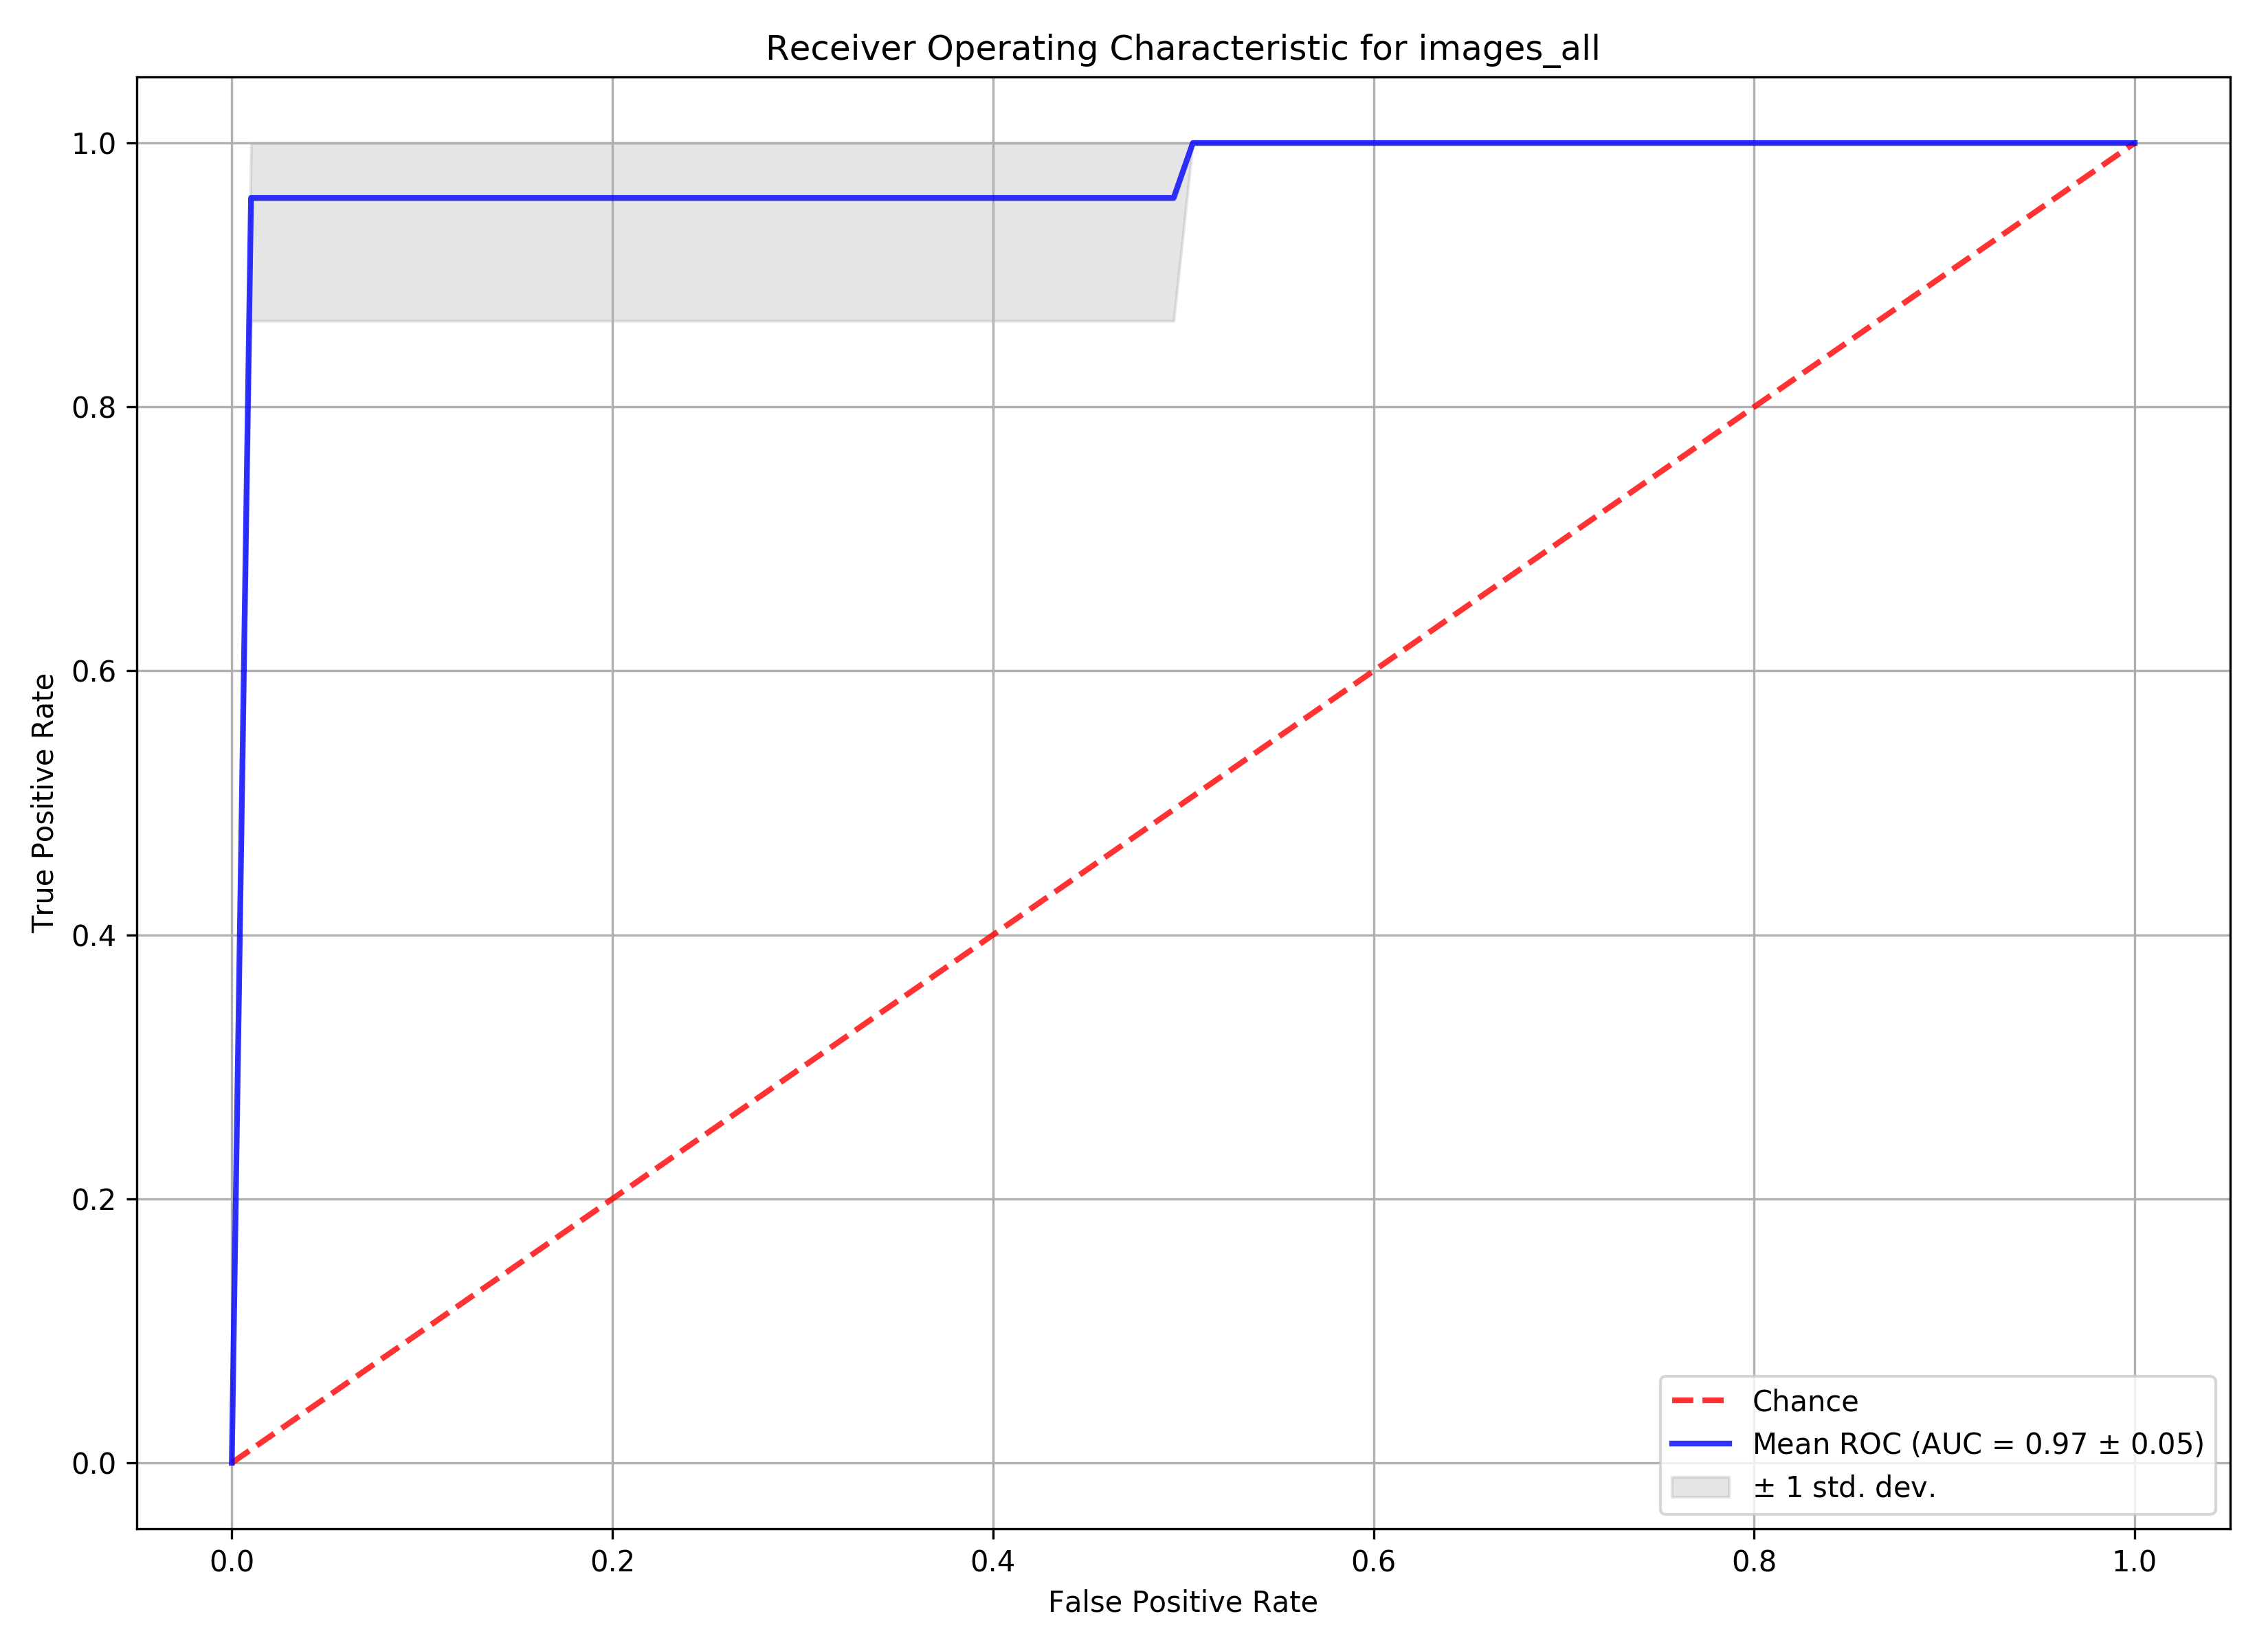
\includegraphics[width=\textwidth,height=\textheight,keepaspectratio]{../Chap4/Figures/roc_images_all_224_3cams_densenet_conv4_PCA20.png}
	\caption{Courbe ROC du meilleur classifieur de la qualité des pièces pour l'essai "boîtes noires".}
	\label{fig:roc_result}
\end{figure}

Cette courbe permet de choisir la valeur optimale de séparation entre les deux classes en fonction de la probabilité de conformité retournée par le réseau.
Dans notre cas, une valeur milieu de $0,5$ est satisfaisante.
On observe également que l'écart-type obtenu par la validation croisée \textit{3-folds} est très faible.
Le système de classification de la qualité est ici très performant. 

\subsubsection{Analyse non-supervisée}
Afin de poursuivre l'analyse, nous avons réalisé une Analyse en Composantes Principales (ACP)\footnote{Le principe de l'Analyse en Composantes Principales est détaillé dans la Section \ref{subsubsec:ACP}.} à partir de la réduction \textit{UMAP}\footnote{L'algorithme de réduction de dimension non-supervisé \textit{UMAP} est discuté dans la Section \ref{subsubsec:umap}.} à cent scalaires de la dernière couche \textit{FC2} du réseau (564 valeurs scalaires réduites à cent scalaires).
Le code couleur représente en vert les pièces conformes, en rouge les pièces non-conformes. L'interface utilisateur permet d'afficher l'image associée à chacun des points lors du survol ou du clic.
La Figure \ref{fig:umap_box} présente le résultat obtenus à l'aide des trois composantes principales.
Cette représentation est disponible dans l'interface utilisateur que nous avons développée ; le survol à la souris de chacun des points affiche l'image associée, ce qui permet de valider les performances.
% Analyse en Composantes Principales réalisée sur une réduction de la dimension des images des quatre caméras à 100 valeurs scalaires à l'aide de l'algorithme UMAP (présenté dans le chapitre précédent à la Section \ref{subsubsec:umap}).

\begin{figure}[tbhp]
	\centering
	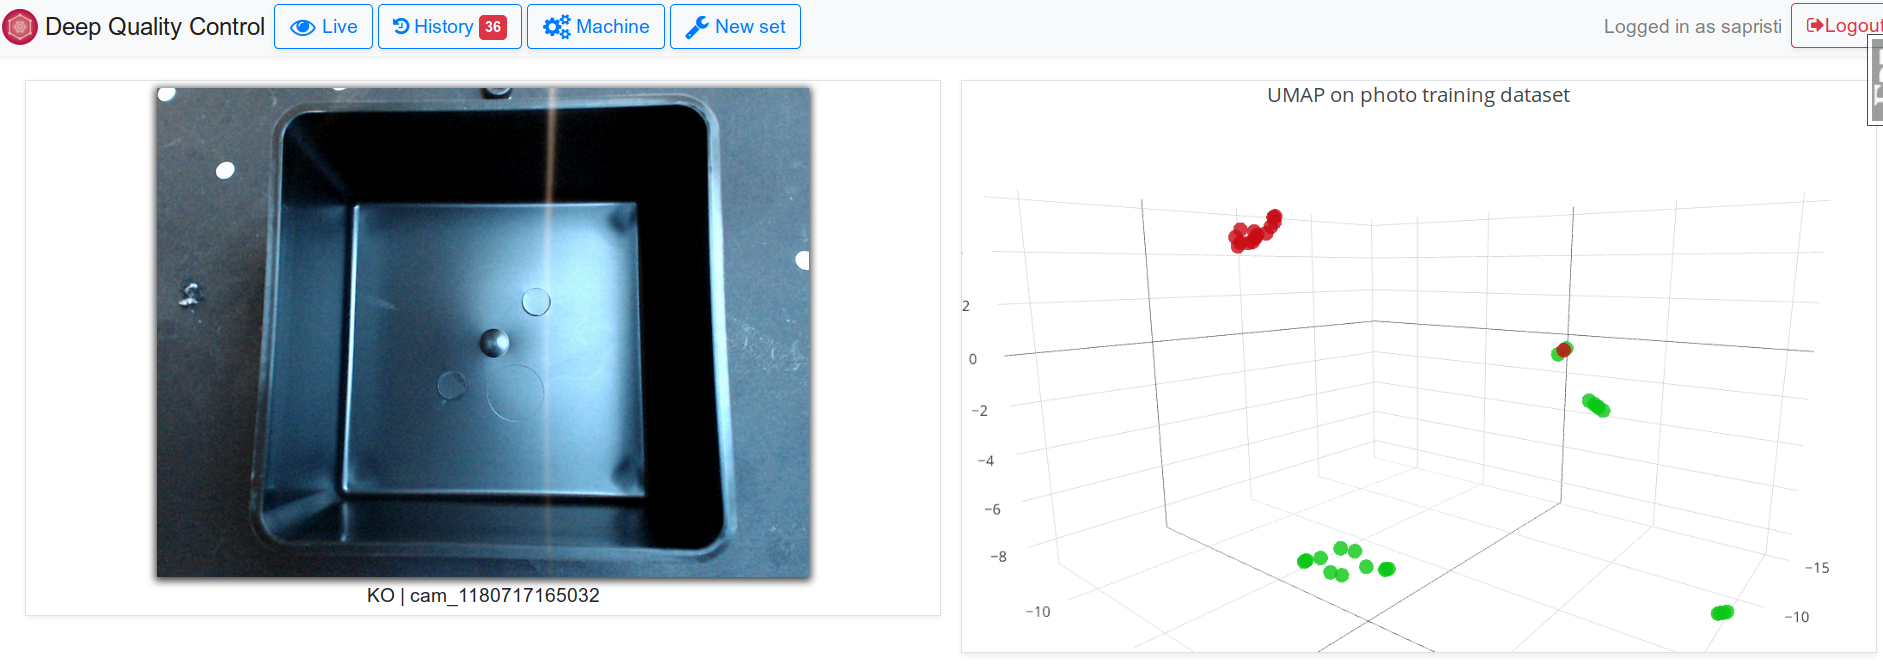
\includegraphics[width=\textwidth,height=\textheight,keepaspectratio]{../Chap5/Figures/Capture-2018-11-21-15-12-07.png}
	\caption{ACP sur réduction \textit{UMAP} à 100 scalaires des 564 valeurs de la dernière couche du réseau.}
	\label{fig:umap_box}
\end{figure}

On observe que les pièces conformes sont bien séparées des pièces non-conformes.
De plus, une pièce non-conforme (de couleur rouge) est située à proximité d'un lot de pièces conformes : c'est une erreur d'annotation de l'humain.
Enfin, on observe que l'information issue de la dernière couche du réseau permet de discrétiser différentes catégories de pièces conformes.
Une étude par clustering non-supervisé (discuté dans la Section \ref{subsec:unsupervised}) permettrait d'enrichir les informations données par notre système en donnant les catégories de pièce, en plus de la classification de non-conformité binaire.

\subsubsection{Cartes de saillance}
Afin d’interpréter les résultats obtenus en classification par les réseaux de convolution profonds, il est possible de construire une carte de saillance\footnote{Les cartes de saillance sont issues de la méthode de réduction de dimensions par interpolation (le \textit{pooling}) qui est utilisée dans les réseaux de convolutions profonds. Nous discutons de la mise en œuvre de ces cartes dans l'Annexe \ref{parag:pooling}.} des pixels de l'image qui ont été important pour réaliser la classification.
Cette carte est construite en sommant les valeurs des pixels de l’image pour chaque couche d’activation du réseau profond \cite{simonyan_deep_2013, li_visual_2015}.
Nous utilisons deux algorithmes pour réaliser ces cartes : (a) la rétro-propagation guidée \cite{springenberg_striving_2014} avec régularisation \cite{smilkov_smoothgrad_2017} et (b) l’algorithme \textit{Grad-CAM} \cite{selvaraju_grad-cam_2016}.
Nous avons adapté la librairie \textit{keras-viz} à nos données \cite{raghakotkerasvis}.

La Figure \ref{fig:saliency} présente ces cartes obtenues pour une pièce conforme et une pièce non-conforme.
Nous avons réalisé la carte de saillance pour l'image dont la polarisation linéaire est de 0° par rapport à l'éclairage annulaire.
Les pixels saillants de l’image, pour le réseau de neurones, sont les bords de la pièce où se situent les défauts géométriques, ainsi que les régions planes où apparaissent des défauts d’aspect.
% Le réseau prend donc en compte, en priorité, ces éléments pour inférer la conformité.
Ces cartes montrent que le réseau de neurones a appris à s'intéresser aux éléments de la pièce pour inférer la conformité.
% Ces cartes appuient la pertinence de la méthode employée.

\begin{figure}[hb!]
	\centering
	\begin{subfigure}[c]{0.63\textwidth}
		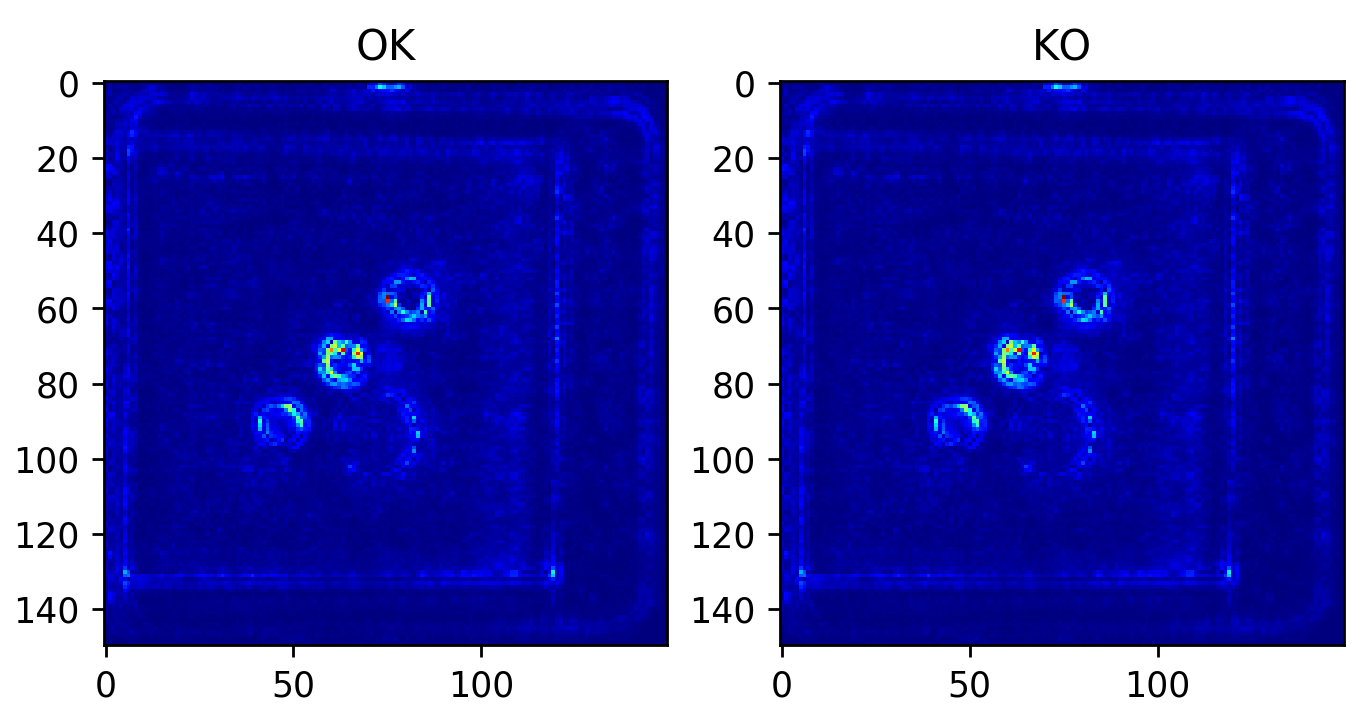
\includegraphics[width=\textwidth]{../Chap5/Figures/visualize_saliency_more_guided.png}
		\caption{Carte de saillance par l'algorithme "\textit{guided backpropagation}".}
	\end{subfigure}
	\\
	\bigskip
	\begin{subfigure}[c]{0.63\textwidth}
		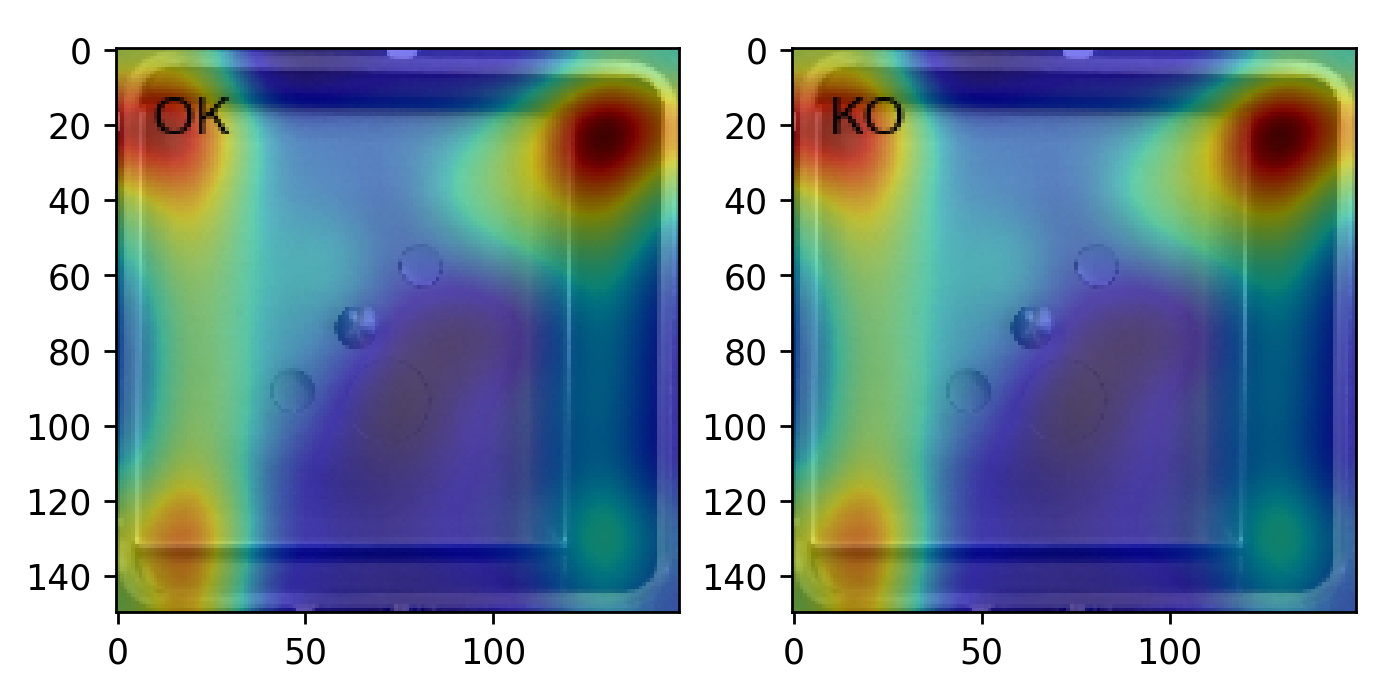
\includegraphics[width=\textwidth]{../Chap5/Figures/visualize_saliency_grad-CAM_relu.png}
		\caption{Carte de saillance par l'algorithme "\textit{grad-CAM}".}
	\end{subfigure}
	\caption{Cartes de saillance obtenues pour une pièce conforme et une pièce non-conforme.}
	\label{fig:saliency}
\end{figure}

% \newpage
\subsection{Essai "plaques" confidentiel}
% ProtoOct18-crop.jpg
Dans la cadre du projet de recherche collaboratif FUI SAPRISTI, nous avons réalisé un essai chez un industriel en Avril 2019.
Le cadre et les résultats de cet essai sont confidentiels.
Ils sont détaillés dans l'Annexe \ref{Ann:plaques}.

% \newpage
\subsection{Discussions et limites du système proposé}
Les essais expérimentaux nous permettent de mettre en évidence les limites qui apparaissent sur notre système.
Le premier cas d'application "boîte noire" montre des résultats très encourageants.
En revanche, le second cas d'application n'est pas satisfaisant.
Il montre la difficulté à réaliser un système capable de contrôler tous types de pièces.
Dans cette section, nous discuterons de principales limites de notre système.

\subsubsection{Faible nombre d'échantillons dans les essais expérimentaux}
Le nombre de pièces dans les jeux de données des essais expérimentaux est très faible en comparaison des milliers d’échantillons généralement présentés dans la littérature de l'apprentissage statistique.
L'augmentation artificielle du jeu de données par transformation aléatoire des images que nous utilisons ne permet pas de remplacer l'acquisition de nouvelles données réelles.
% Il est possible qu’un biais existe dans nos jeux de données.
Nous espérons éprouver dans l'avenir notre système sur une quantité de données plus importante.
Cela permettra de justifier notre approche et d'identifier les biais potentiels.

\subsubsection{Répétabilité du positionnement}
Une difficulté importante a été identifiée lors du second essai "plaques".
La pièce était déposée par le robot sur un tapis avant son contrôle.
Cette opération introduit une variation du positionnement des pièces.
Les traitements d'image pour compenser ces variations que nous avons réalisés ne ce sont pas montrées suffisantes.
Cette variabilité dans le positionnement introduit un biais dans le jeu de données.
En pratique, il est préférable que le positionnement des pièces soit répétable pour supprimer cette cause de biais.
Le positionnement par un posage précis de la pièce ou par la répétition d'un bras robotisé est recommandé.
Le bras robotisé a été utilisé avec succès dans le premier essai "boîtes noires".
% Enfin, une piste possible est de mettre en place un référentiel de positionnement absolue en attachant sur le bras robotoque des marqueurs de référence qui permettront de compenser les variations par homographie.

% Problème : voir des micro-variations, maitriser le positionnement
% Difficulté de stabilisation par homographie ou optical flow.
% Maurice : il faut que l’image soit identique au pixel prêt. Posage.
% Émilio : tjs une incertitude de positionnement. La prise d’image doit avoir lieu quand le robot a la pièce. Le robot présente la pièce à la mesure, avant le dépôt sur le convoyeur.
% Maurice : référentiel sur le bras robotique (3, 4 points) pour recaler.
% Maurice : Attention d’une série à l’autre le banc de mesure peut bouger !

\subsubsection{Limites de la solution de capture retenue}
Notre système est limité à un unique point de vue.
Pour notre cas d'étude, les surfaces à évaluer des pièces sont situées dans un même plan.
Dans le cas de pièces courbes, il serait intéressant d’utiliser notre méthode en multipliant le nombre de points de vues : deux caméras pour couvrir 270 degrés d’angle de champ et trois caméras pour une révolution complète.
Enfin, il serait intéressant d’évaluer la dégradation de performance de la classification de la qualité en fonction de la définition du capteur.
Notre prototype utilise de simples webcams grands publics, mais des solutions de caméras industrielles de meilleurs résolutions existent à des coûts plus élevés.


% \begin{raggedright}
% 	\section{Évaluation de la performance du système de mesure de la Qualité}
% \end{raggedright}
% Coût industrielle de la non-qualité
% \subsection{Comparaison avec un expert humain}
% TODO: Gage R et R avec expert humain
% \subsection{Métrique de confidence industrielle}
% TODO: faux positif, faux négatif, ppm
% Limite au déploiement : 2-3 x meilleur qu'un humain
% Coût industriel de la non-qualité vs coût du déploiement d'un tel système, fonction de la valeur ajouté du produit
% À propos des attaques par exemple adversaire : détecter l'attaque.

\newpage
\section{Conclusion}
\vspace{-3mm}
Dans ce chapitre, nous avons présenté notre proposition d'un système de contrôle de la qualité en ligne de production, à partir d'images non-conventionnelles.
Le système utilise une architecture client-serveur et un réseau de neurones profonds pour extraire et fusionner l'information de plusieurs caméras.
Le réseau de neurones permet d'adapter le système à chaque type de pièce, par apprentissage.

Le réseau de neurones retourne une probabilité de conformité de la pièce.
La valeur de cette probabilité est utilisée à l'aide d'un seuil, pour définir si la pièce est conforme ou non.
En fonction de l'application, il est possible de limiter le nombre de pièces non-conformes dans le lot final en augmentant le seuil du nombre de pièces conformes qui sont classées comme non-conformes (faux négatifs).
Cette démarche augmente les rebuts mais permet de limiter le risque de pièces non-conformes dans le lot final.

Une interface utilisateur, dans un navigateur web, permet à l'utilisateur, technicien-régleur ou expert qualité, d'apprendre au système à reconnaître les pièces conformes ou non.
Chaque nouvelle pièce, enregistrée par le système, est affichée dès sa prise de vue.
L'interface affiche le degré de conformité retourné par le système et l'utilisateur peut modifier la réponse donnée si celle-ci est erronée.
Toutes les vingts nouvelles pièces annotées, le modèle est mis à jour.

Nous avons réalisé deux essais expérimentaux afin d'évaluer les performances du système.
L'essai "boîtes noires" présente de très bons résultats de classification.
En revanche, l'essai "plaques" présente des résultats peu satisfaisants.
Le manque de répétabilité du positionnement des pièces, lors de la mesure, a introduit un biais dans le jeu de données.
Suite à cet essai, nous recommandons de mettre en place un positionnement répétable, si possible au pixel prêt, à l'aide d'un posage ou d'un bras robotisé.

La principale suite à ces travaux est la validation des performances sur un plus grand nombre d'individus.
Actuellement, les résultats sont obtenus sur des productions de plusieurs centaines de pièces.
% Un nombre d'échantillon supérieur à mille permettrait d'avoir une confidence plus élevée.
L'acquisition massive de données permettrait également d'améliorer le modèle par apprentissage.
De plus, la réponse des réseaux de neurones profonds gagnent en robustesse lorsque les individus du jeu de données sont variés.

\vspace{-15mm}
\section{Perspectives}
%Afin de réaliser ces perspectives, nous proposons de :
%- maximiser l'adoption
%- commercialisation pas chère = récupérer un maximum de données pour améliorer les modèles.
%- voir même commercialisation gratuite pour maximiser la récolte de données.
% Plusieurs perspectives de recherche sont envisagées afin d'évaluer notre système.
\vspace{-3mm}
% \subsection{Validation sur de multiples cas d'application}
\paragraph{3.4.1 Validation sur de multiples cas d'application} \mbox{} \\
La mise à disposition d'un système de qualification mobile et intégré permet d'envisager la réalisation de nombreux essais sur des lignes de production.
L'objectif sera de multiplier les cas d'application afin de valider les performances et d'optimiser les traitements.
Il sera également intéressant d'évaluer notre système sur d'autres procédés de fabrication.
En particulier, d'autres procédés qui produisent des pièces chaudes ou qui possèdent une variabilité de la thermique seront intéressant à étudier.
\vspace{-4mm}
% \subsection{Apprentissage semi et non-supervisé}
\paragraph{3.4.2 Apprentissage semi et non-supervisé} \mbox{} \\
Enfin, l'intérêt des approches semi-supervisés et non-supervisés est de se passer de l'expertise humaine pour apprendre le modèle.
En effet, l'expert humain peut introduire un biais dans le jeu de données.
De plus, le travail d'annotation humaine présente un certain coût.
La classification non-supervisée de la conformité permettrait également pour pouvoir classifier la qualité sans donnée initiale, dès la mise en route du système de qualification.
Nous n'avons pas évalué cette approche qui est une perspective importante.
La Section \ref{subsec:semi_supervised} discute des méthodes envisageables et présente des applications qualitatives sur nos données.
En particulier, nous nous intéresserons, en suite directe de ce travail, à l'utilisation des auto-encodeurs variationnels\footnote{Les auto-encodeurs variationnels sont des réseaux génératifs. Nous discutons de leurs utilisations sur nos données dans la Section \ref{subsubsec:vae}.} pour extraire l'information des images de manière non supervisée.
% \begin{enumerate}
% 	\item fusion des données brutes des capteurs,
% 	\item réduction de dimensions VAE / UMAP,
% 	\item clustering HDBSCAN.
% \end{enumerate}

% \subsection{Résultats obtenus par le dispositif de mesure TheEye}
% -> Perspectives, TheEye, nouveaux champs de recherche :
% - à la Qualité, au suivi en temps réel des dérives de la production, à l'ajustement du procédé
% - à d'autres mesures
% - à d'autres sources d'infos
% - à d'autres produits
% -> Apprentissage semi-supervisé et non-supervisé
